%%% File-Information {{{
%%% Filename: template_bericht.tex
%%% Purpose: lab report, technical report, project report
%%% Time-stamp: <2004-06-30 18:19:32 mp>
%%% Authors: The LaTeX@TUG-Team [http://latex.tugraz.at/]:
%%%          Karl Voit (vk), Michael Prokop (mp), Stefan Sollerer (ss)
%%% History:
%%%   20050914 (ss) correction of "backref=true" to "backref" due to hyperref documentation
%%%   20040630 (mp) added comments to foldmethod at end of file
%%%   20040625 (vk,ss) initial version
%%%
%%% Notes:
%%%
%%%
%%%
%%% }}}
%%%%%%%%%%%%%%%%%%%%%%%%%%%%%%%%%%%%%%%%%%%%%%%%%%%%%%%%%%%%%%%%%%%%%%%%%%%%%%%%
%%% main document {{{

\documentclass[
a4paper,     %% defines the paper size: a4paper (default), a5paper, letterpaper, ...
% landscape,   %% sets the orientation to landscape
% twoside,     %% changes to a two-page-layout (alternatively: oneside)
% twocolumn,   %% changes to a two-column-layout
% headsepline, %% add a horizontal line below the column title
% footsepline, %% add a horizontal line above the page footer
% titlepage,   %% only the titlepage (using titlepage-environment) appears on the first page (alternatively: notitlepage)
% parskip,     %% insert an empty line between two paragraphs (alternatively: halfparskip, ...)
% leqno,       %% equation numbers left (instead of right)
% fleqn,       %% equation left-justified (instead of centered)
% tablecaptionabove, %% captions of tables are above the tables (alternatively: tablecaptionbelow)
% draft,       %% produce only a draft version (mark lines that need manual edition and don't show graphics)
% 10pt         %% set default font size to 10 point
% 11pt         %% set default font size to 11 point
12pt         %% set default font size to 12 point
]{scrartcl}  %% article, see KOMA documentation (scrguide.dvi)

%%%%%%%%%%%%%%%%%%%%%%%%%%%%%%%%%%%%%%%%%%%%%%%%%%%%%%%%%%%%%%%%%%%%%%%%%%%%%%%%
%%%
%%% packages
%%%

%%%
%%% encoding and language set
%%%

%%% ngerman: language set to new-german
\usepackage[english]{babel} 
\usepackage{tocloft}
\usepackage{subcaption}
\usepackage{listings}
\usepackage{color} %red, green, blue, yellow, cyan, magenta, black, white
\usepackage{courier}
\usepackage{float}

%%% babel: language set (can cause some conflicts with package ngerman)
%%%        use it only for multi-language documents or non-german ones
%\usepackage[ngerman]{babel}

%%% inputenc: coding of german special characters
\usepackage[latin1]{inputenc}

%%% fontenc, ae, aecompl: coding of characters in PDF documents
\usepackage[T1]{fontenc}
\usepackage{ae,aecompl}

%%%
%%% technical packages
%%%

%%% amsmath, amssymb, amstext: support for mathematics
%\usepackage{amsmath,amssymb,amstext}

%%% psfrag: replace PostScript fonts
\usepackage{psfrag}

%%% listings: include programming code
%\usepackage{listings}

%%% units: technical units
%\usepackage{units}

%%%
%%% layout
%%%

%%% scrpage2: KOMA heading and footer
%%% Note: if you don't use this package, please remove 
%%%       \pagestyle{scrheadings} and corresponding settings
%%%       below too.
\usepackage[automark]{scrpage2}


%%%
%%% PDF
%%%

\usepackage{ifpdf}

%%% Should be LAST usepackage-call!
%%% For docu on that, see reference on package ``hyperref''
\ifpdf%   (definitions for using pdflatex instead of latex)

  %%% graphicx: support for graphics
  \usepackage[pdftex]{graphicx}

  \pdfcompresslevel=9

  %%% hyperref (hyperlinks in PDF): for more options or more detailed
  %%%          explanations, see the documentation of the hyperref-package
  \usepackage[%
    %%% general options
    %pdftex=true,      %% sets up hyperref for use with the pdftex program
    %plainpages=false, %% set it to false, if pdflatex complains: ``destination with same identifier already exists''
    %
    %%% extension options
    backref,      %% adds a backlink text to the end of each item in the bibliography
    pagebackref=false, %% if true, creates backward references as a list of page numbers in the bibliography
    colorlinks=false,   %% turn on colored links (true is better for on-screen reading, false is better for printout versions)
    %
    %%% PDF-specific display options
    bookmarks=true,          %% if true, generate PDF bookmarks (requires two passes of pdflatex)
    bookmarksopen=false,     %% if true, show all PDF bookmarks expanded
    bookmarksnumbered=false, %% if true, add the section numbers to the bookmarks
    %pdfstartpage={1},        %% determines, on which page the PDF file is opened
    pdfpagemode=UseNone         %% None, UseOutlines (=show bookmarks), UseThumbs (show thumbnails), FullScreen
  ]{hyperref}


  %%% provide all graphics (also) in this format, so you don't have
  %%% to add the file extensions to the \includegraphics-command
  %%% and/or you don't have to distinguish between generating
  %%% dvi/ps (through latex) and pdf (through pdflatex)
  \DeclareGraphicsExtensions{.pdf}

\else %else   (definitions for using latex instead of pdflatex)

  \usepackage[dvips]{graphicx}

  \DeclareGraphicsExtensions{.eps}

  \usepackage[%
    dvips,           %% sets up hyperref for use with the dvips driver
    colorlinks=false %% better for printout version; almost every hyperref-extension is eliminated by using dvips
  ]{hyperref}

\fi


%%% sets the PDF-Information options
%%% (see fields in Acrobat Reader: ``File -> Document properties -> Summary'')
%%% Note: this method is better than as options of the hyperref-package (options are expanded correctly)
\hypersetup{
  pdftitle={Image Based Measurement Laboratory 1}, %%
  pdfauthor={Filzmaier Josef, Michael Sieberer}, %%
  pdfsubject={Image Stitching, Auto-Focus, Sensor Dynamics, Perspective invariants}, %%
  pdfcreator={Accomplished with LaTeX2e and pdfLaTeX with hyperref-package.}, %% 
  pdfproducer={}, %%
  pdfkeywords={} %%
}


%%%%%%%%%%%%%%%%%%%%%%%%%%%%%%%%%%%%%%%%%%%%%%%%%%%%%%%%%%%%%%%%%%%%%%%%%%%%%%%%
%%%
%%% user defined commands
%%%

%%% \mygraphics{}{}{}
%% usage:   \mygraphics{width}{filename_without_extension}{caption}
%% example: \mygraphics{0.7\textwidth}{rolling_grandma}{This is my grandmother on inlinescates}
%% requires: package graphicx
%% provides: including centered pictures/graphics with a boldfaced caption below
%% 
\newcommand{\mygraphics}[3]{
  \begin{center}
    \includegraphics[width=#1, keepaspectratio=true]{#2} \\
    \textbf{#3}
  \end{center}
}

%%%%%%%%%%%%%%%%%%%%%%%%%%%%%%%%%%%%%%%%%%%%%%%%%%%%%%%%%%%%%%%%%%%%%%%%%%%%%%%%
%%%
%%% define the titlepage
%%%

% \subject{}   %% subject which appears above titlehead
% \titlehead{} %% special heading for the titlepage

%%% title
\title{Image Based Measurement Laboratory\\\vspace{1cm}\Large{Lab1 - Uncalibrated Sensors}}

%%% author(s)
\author{Filzmaier Josef (1030462) \and
Michael Sieberer (1531366)}

%%% date
\date{Graz, am \today{}}

% \publishers{}

% \thanks{} %% use it instead of footnotes (only on titlepage)

% \dedication{} %% generates a dedication-page after titlepage


%%% uncomment following lines, if you want to:
%%% reuse the maketitle-entries for hyperref-setup
%\newcommand\org@maketitle{}
%\let\org@maketitle\maketitle
%\def\maketitle{%
%  \hypersetup{
%    pdftitle={\@title},
%    pdfauthor={\@author}
%    pdfsubject={\@subject}
%  }%
%  \org@maketitle
%}


%%%%%%%%%%%%%%%%%%%%%%%%%%%%%%%%%%%%%%%%%%%%%%%%%%%%%%%%%%%%%%%%%%%%%%%%%%%%%%%%
%%%
%%% set heading and footer
%%%

%%% scrheadings default: 
%%%      footer - middle: page number
\pagestyle{scrheadings}

%%% user specific
%%% usage:
%%% \position[heading/footer for the titlepage]{heading/footer for the rest of the document}

%%% heading - left
% \ihead[]{}

%%% heading - center
% \chead[]{}

%%% heading - right
% \ohead[]{}

%%% footer - left
% \ifoot[]{}

%%% footer - center
% \cfoot[]{}

%%% footer - right
% \ofoot[]{}

\renewcommand*{\thesection}{Exercise~\arabic{section}:}
\renewcommand*{\thesubsection}{\arabic{section}.\arabic{subsection}}
\setlength{\cftsecnumwidth}{6.0em}
\setlength\parindent{0pt}
\definecolor{mygreen}{RGB}{28,172,0} % color values Red, Green, Blue
\definecolor{mylilas}{RGB}{170,55,241}
\lstset{language=Matlab,%
    basicstyle=\ttfamily\footnotesize,breaklines=true,
    breaklines=true,%
    morekeywords={matlab2tikz},
    keywordstyle=\color{blue},%
    morekeywords=[2]{1}, keywordstyle=[2]{\color{black}},
    identifierstyle=\color{black},%
    stringstyle=\color{mylilas},
    commentstyle=\color{mygreen},%
    showstringspaces=false,%without this there will be a symbol in the places where there is a space
    numbers=left,%
    numberstyle={\tiny \color{black}},% size of the numbers
    numbersep=9pt, % this defines how far the numbers are from the text
    emph=[1]{for,end,break},emphstyle=[1]\color{red}, %some words to emphasise
    captionpos=b,
    %emph=[2]{word1,word2}, emphstyle=[2]{style},    
}
\newcommand{\sidebysidepic}[6]{
\begin{figure}[ht!]%
\begin{subfigure}{.5\textwidth}%
  \centering%
  \includegraphics[width=.8\linewidth]{#1}%
  \caption{#2}%
\end{subfigure}%
\begin{subfigure}{.5\textwidth}%
  \centering%
  \includegraphics[width=.8\linewidth]{#3}%
  \caption{#4}%
\end{subfigure}%
\caption{#5}%
\label{#6}%
\end{figure}%
}

%%%%%%%%%%%%%%%%%%%%%%%%%%%%%%%%%%%%%%%%%%%%%%%%%%%%%%%%%%%%%%%%%%%%%%%%%%%%%%%%
%%%
%%% begin document
%%%

\begin{document}

% \pagenumbering{roman} %% small roman page numbers

%%% include the title
% \thispagestyle{empty}  %% no header/footer (only) on this page
 \maketitle

%%% start a new page and display the table of contents
 \tableofcontents
 \newpage

\section{Image stitching}

\subsection{Problem statement}

Shoot two consecutive pictures containing the target and combine them into a single image. Make use of the
target to define point correspondences, which were used to calculate an according homography. The MATLAB
function \texttt{PanoramaStiching.m} is provided and displays the stitched image given the two images and extracted
correspondences.

\begin{itemize}
 \item Try different numbers of point correspondences.
 \item Vary the distance between selected corners (i.e. select corners near each border of the target. Next time choose four corners placed around a single square).
 \item Why are some correspondences better than others? How can certain differences along the line of intersection be explained? Compare and discuss your results.
\end{itemize}

\subsection{Solution}

Two images from two different perspectives containing a target are taken with two different cameras.
Figure \ref{fig:photo12.5mm} shows the photos taken with a focus length of $12.5mm$ while Figure \ref{fig:photo6.5mm} shows the photos taken with a focus length of $6.5mm$.
The target is the chess board seen in both pictures of each focal length.

\sidebysidepic{./Bildg_Messtechnik_Lab/PanoramaStitching/images/image_1.png}
{First perspective}
{./Bildg_Messtechnik_Lab/PanoramaStitching/images/image_2.png}
{Second perspective}
{Images capturing target from different perspectives with $12.5mm$ focal length}
{fig:photo12.5mm}

\sidebysidepic{./Bildg_Messtechnik_Lab/PanoramaStitching/images/image_b1.png}
{First perspective}
{./Bildg_Messtechnik_Lab/PanoramaStitching/images/image_b2.png}
{Second perspective}
{Images capturing target from different perspectives with $6.5mm$ focal length}
{fig:photo6.5mm}

Corners within the chess board were chosen as unique locations to stitch the two images.
At first four unique image locations within the target are chosen in the first image.
The corresponding points within the second image are chosen directly afterwards.
Listing \ref{lst:panoramastitching} shows the implementation of the task in MatLab.
The function \lstinline{PanoramaStitching(...)} shown at the end in Listing \ref{lst:panoramastitching} is the heart of the algorithm.
It uses the positional information of the four points to calculate a distorted version of image two and moves it to match the points of image one.

\lstinputlisting[caption=Matlab Code, label=lst:panoramastitching]{./Bildg_Messtechnik_Lab/PanoramaStitching/main.m}

There are several options to choose the points within the target.
Some ideas and its results are discussed in the following sections.

\subsubsection{All points are corresponding within the target over a large area}

At first a very obvious choice is taken: Use four corner points of the target in each image.
The results of this approach are quite impressive.
Figure \ref{fig:largeareastitch} shows that the two images are matching very well.
The chosen points can be seen within the target marked as red.
This can especially be seen on the edges of the concrete wall where the target is mounted as they are fitting almost perfectly over their whole length.
When looking at the tripod to the right one can see that distortion gets larger the further away from the image middle we analyse.
The tripod looks like it has a small crack.
Also one can recognize some color mismatch at the stitching points which is to be expected when taking pictures from different angles without calculating som sort of mean value for the colors.

\sidebysidepic{./Bildg_Messtechnik_Lab/PanoramaStitching/fig1.png}
{$12.5mm$}
{./Bildg_Messtechnik_Lab/PanoramaStitching/figb1.png}
{$6.5mm$}
{Stitched image with points chosen over large area}
{fig:largeareastitch}

\subsubsection{All points are corresponding within the target over a small area}

As a second experiment we chose the points very close together.
The proximity of the points can be seen within figure Figure \ref{fig:smallareastitch}, as they just surround one black square within the target.
This approach results in a much more varying scenario.
Discretizing errors of the camera are much smaller when focussing on a larger area then they are in smaller areas.
When getting faulty information the \lstinline{PanoramaStiching(...)} algorithm can not perform as well as it does with higher qualtiy information.
Therefore the edges are not matching as well.

\sidebysidepic{./Bildg_Messtechnik_Lab/PanoramaStitching/fig2.png}
{$12.5mm$}
{./Bildg_Messtechnik_Lab/PanoramaStitching/figb2.png}
{$6.5mm$}
{Stitched image with points chosen over small area}
{fig:smallareastitch}

\subsubsection{One of the points is chosen differently in image two}

Next up is an experiment where we deliberately chose one point wrong.
In this case the algorithm distorts the image in a way which is obviously wrong.
The results can be seen in Figure \ref{fig:differentareastitch}.
As we chose to move the lower left point further to the right then we were supposed to, the algorithm distorted the second image in a similar way.
The bottom part of the image was clinched while the top part looks like they would be fitting pretty nicely, as the top points were chosen rightfully.

\sidebysidepic{./Bildg_Messtechnik_Lab/PanoramaStitching/fig3.png}
{$12.5mm$}
{./Bildg_Messtechnik_Lab/PanoramaStitching/figb3.png}
{$6.5mm$}
{Stitched image with points chosen over small area}
{fig:differentareastitch}

\subsubsection{An arbitrary constellation of corresponding points}

The last two experiments were only performed with the $6.5mm$ focus length camera.
A seemingly arbitrary but in both cases equally chosen set of points is used to calculate the stitch.
Figure \ref{fig:arbitraryareastitch} shows the result.
The image is stretched a bit too much in its bottom part which is due to discretizing errors of the camera, but otherwise the result looks quite good.

\begin{figure}[ht!]
 \centering
 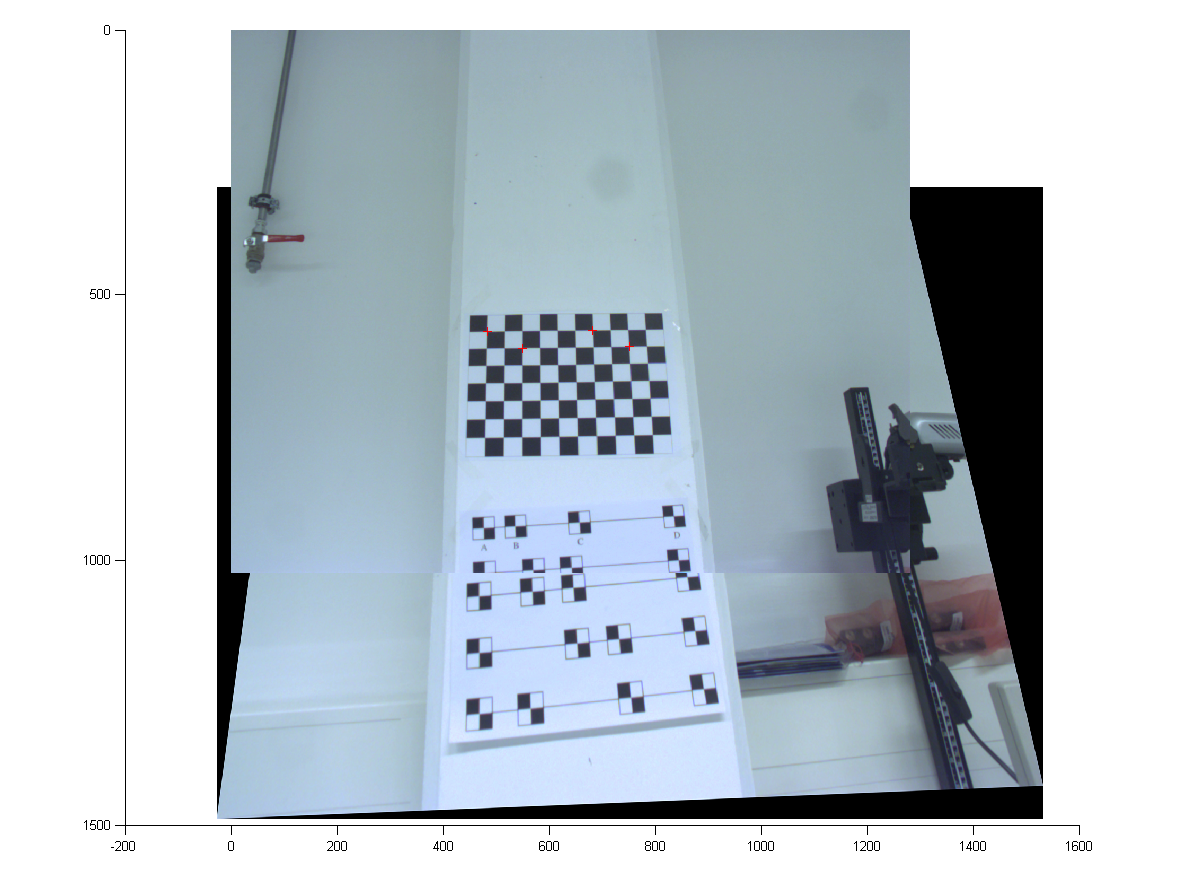
\includegraphics[scale=0.4]{./Bildg_Messtechnik_Lab/PanoramaStitching/figb4.png}
 \caption{Stitched image with arbitrary points ($6.5mm$)}
 \label{fig:arbitraryareastitch}
\end{figure}

\subsubsection{All points are on one line except for one}

At last all points are chosen within a line in the first image while in the second image the last one is chosen very far to the right.
The algorithm produces a radially distorted image (See Figure  \ref{fig:lineareastitch}) probably because it is trying to match the last two points which do not correspond at all.

\begin{figure}[ht!]
 \centering
 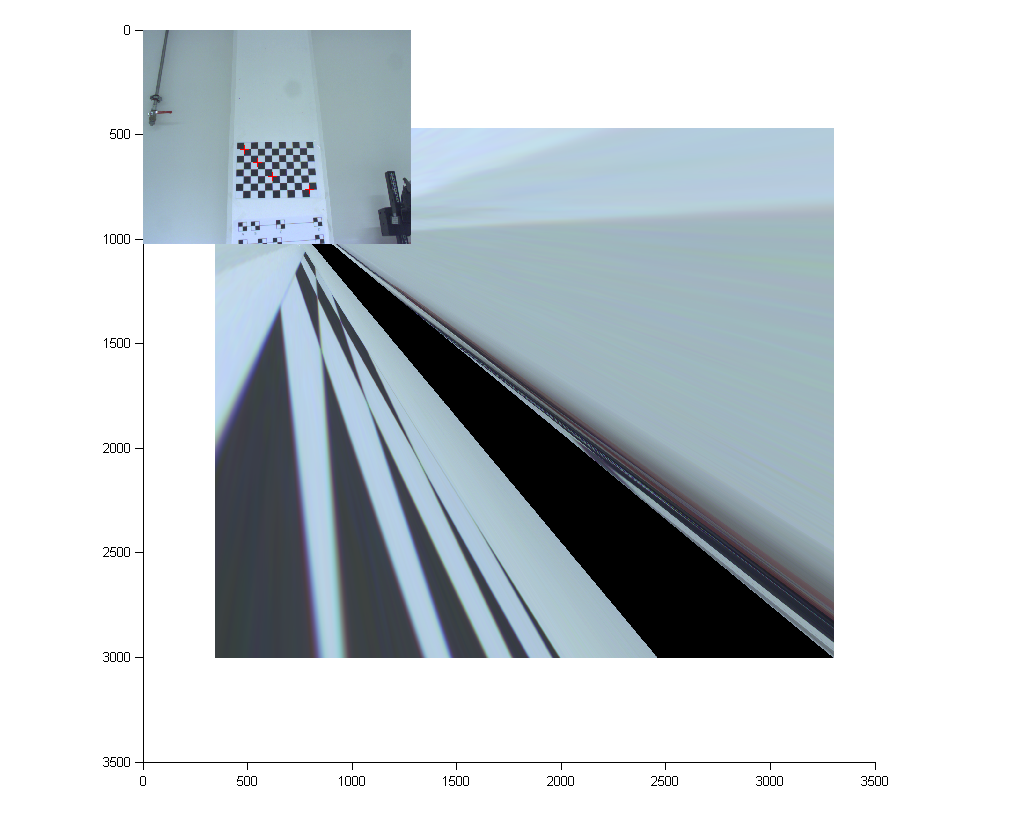
\includegraphics[scale=0.4]{./Bildg_Messtechnik_Lab/PanoramaStitching/figb5.png}
 \caption{Stitched image with points in a line except for one ($6.5mm$)}
 \label{fig:lineareastitch}
\end{figure}

\pagebreak

\section{Auto Focus}

\subsection{Problem statement}

Take a sequence of about $N = 10$ images of a static scene using a linearly varying focus parameter of the
provided camera. Determine scene properties which make the scene well suited for an auto-focus algorithm.
Develop a MATLAB script to determine the best focus image out of this sequence. Repeat your analysis with
different image sequences and discuss your results.

\subsection{Solution}

In order to solve this task we implemented the following four-step idea for all $N$ images:

\begin{itemize}
 \item Convert the colored image to the corresponding grey value image
 \item Calculate the histogram of the grey value image
 \item Sort the histogram values decreasingly
 \item Sum up the first $1000$ elements of the sorted histogram and normalize
\end{itemize}

Figure \ref{fig:alltakenimages} shows a grid of the $N=10$ taken images of the scene with varying focus.
Listing \ref{lst:autofocus} shows the implementation we did end up with.
All lines of code before line 12 are for initializing the computation.
The for loop on line $12$ then iterates over all the $N=10$ input images which were taken in the lab.
In line $15$ the Matlab function for converting the colored image into its grey values is called.
We did this so that we do not have to cope with all three color channels and the result should not be dependent on the colors.
The most important function call is in line $18$ which calculates the gradient of the image using the ``CentralDifference'' algorithm.
Using the gradient image we can determine how sharp edges are within the image.
We then sort the values in descending order in line $20$ and store them within the \lstinline{focVal} variable.

\begin{lstlisting}[label=lst:autofocus, caption=Matlab script for calculating best focus value]
N = 1000;

% directory that contains the image sequence
img_dir = 'images';
img_type = '.png';
img_names = dir([img_dir '/*' img_type]);

imshowD = @(img) imshow(im2uint8(img));
focVal = [];
focName = [];

for i = 1:length(img_names)
    img_name = img_names(i).name;
    img = imread([img_dir '/' img_name]);
    imgG = rgb2gray(img);
    imgG = im2double(imgG);
    
    [grd,~] = imgradient(imgG,'CentralDifference');
    
    grdS = sort(grd,'descend');
    
    focusInd = sum(grdS(1:N)) / N;
    fprintf('%s - %d\n', img_name, focusInd);
    
    focVal = [focVal, focusInd];
end
\end{lstlisting}

Figure \ref{fig:autofocus_hist} clearly shows that the image with the best focus is the image with a focus of $3mm$.
When comparing all the images this result satisfied our expectations as we already beforehand considered that this picture looks like it is best focussed one.

\begin{figure}[ht!]
 \centering
 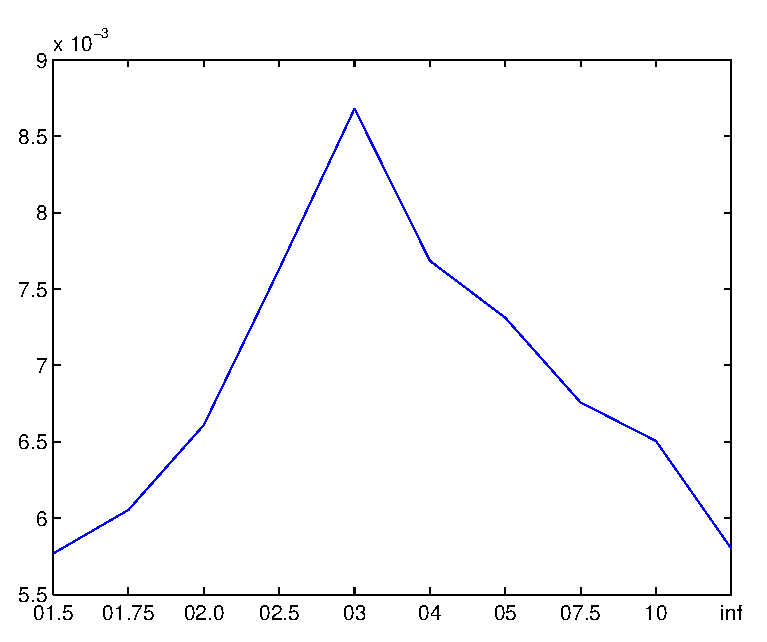
\includegraphics{./Bildg_Messtechnik_Lab/Autofokus/html/main_01.eps}
 \caption{Overview over the calculated focus value for all Images}
 \label{fig:autofocus_hist}
\end{figure}


\begin{figure}
\centering
\begin{tabular}{ccc}
 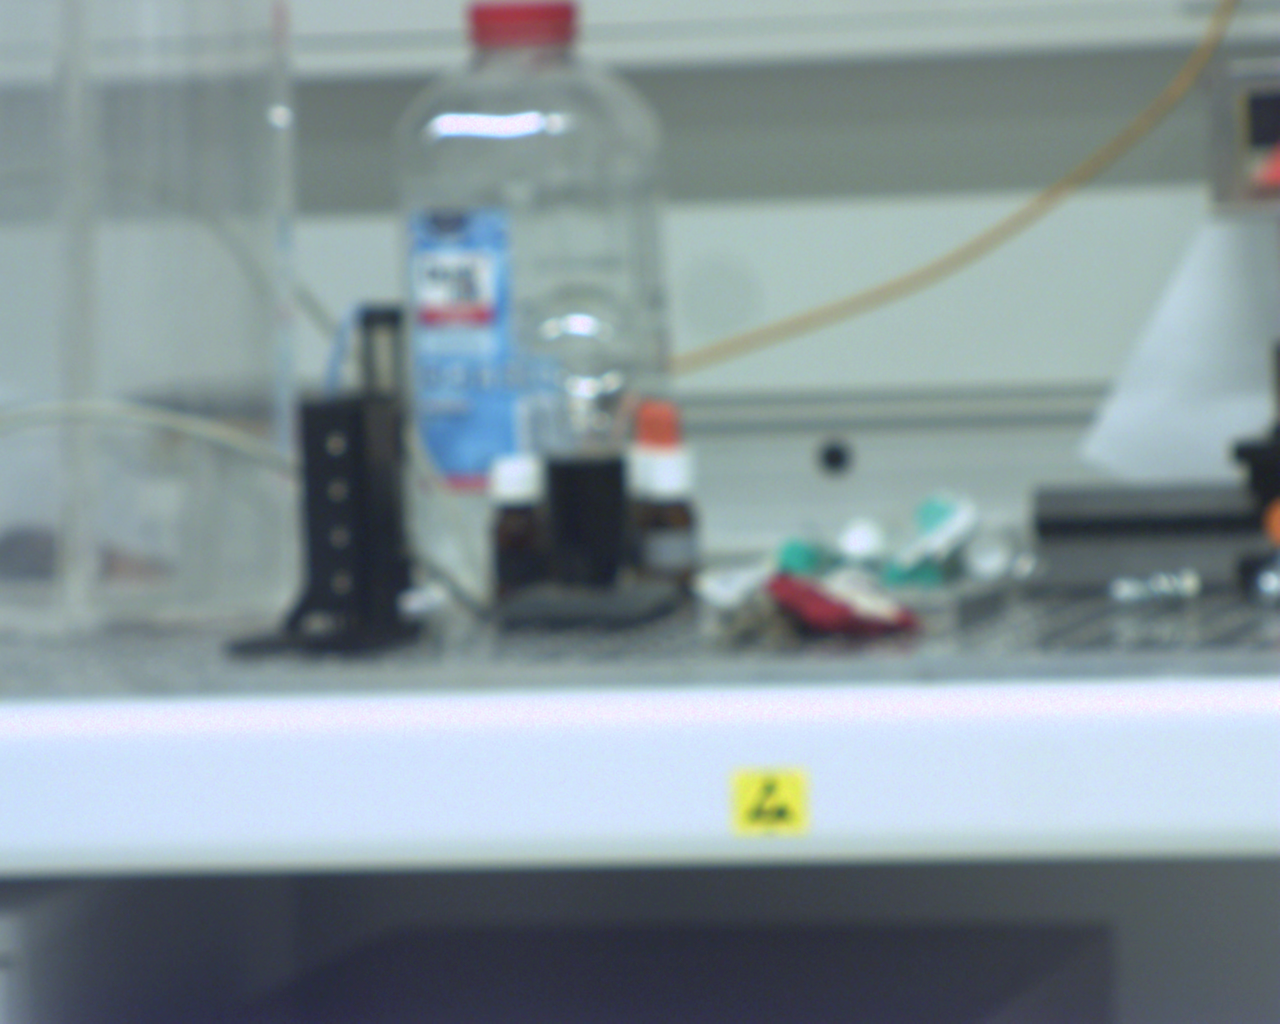
\includegraphics[width=48mm]{./Bildg_Messtechnik_Lab/Autofokus/images/image_01_5.png} & 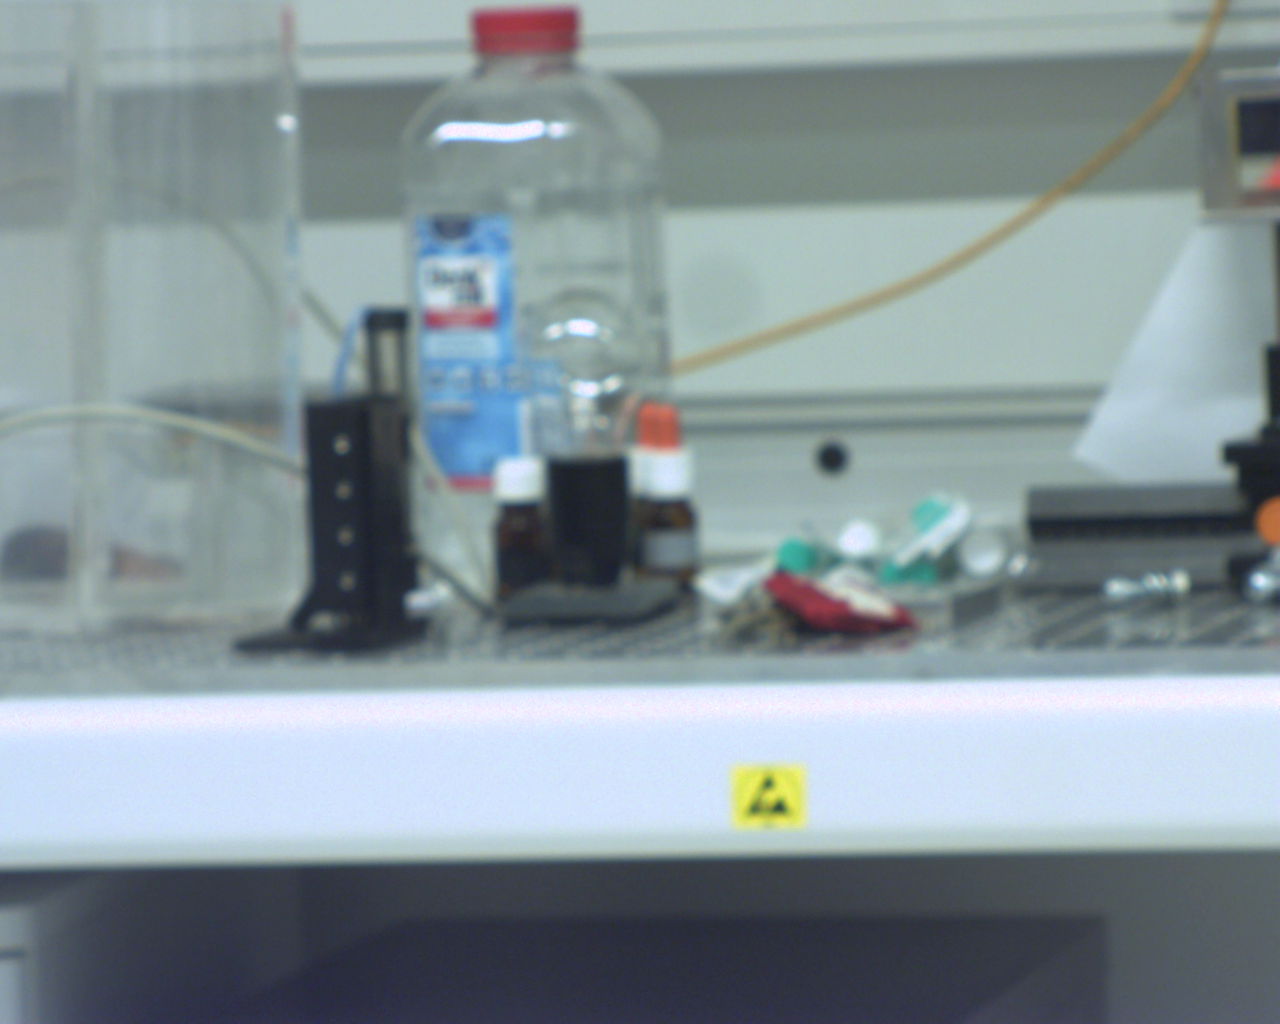
\includegraphics[width=48mm]{./Bildg_Messtechnik_Lab/Autofokus/images/image_01_75.png} & 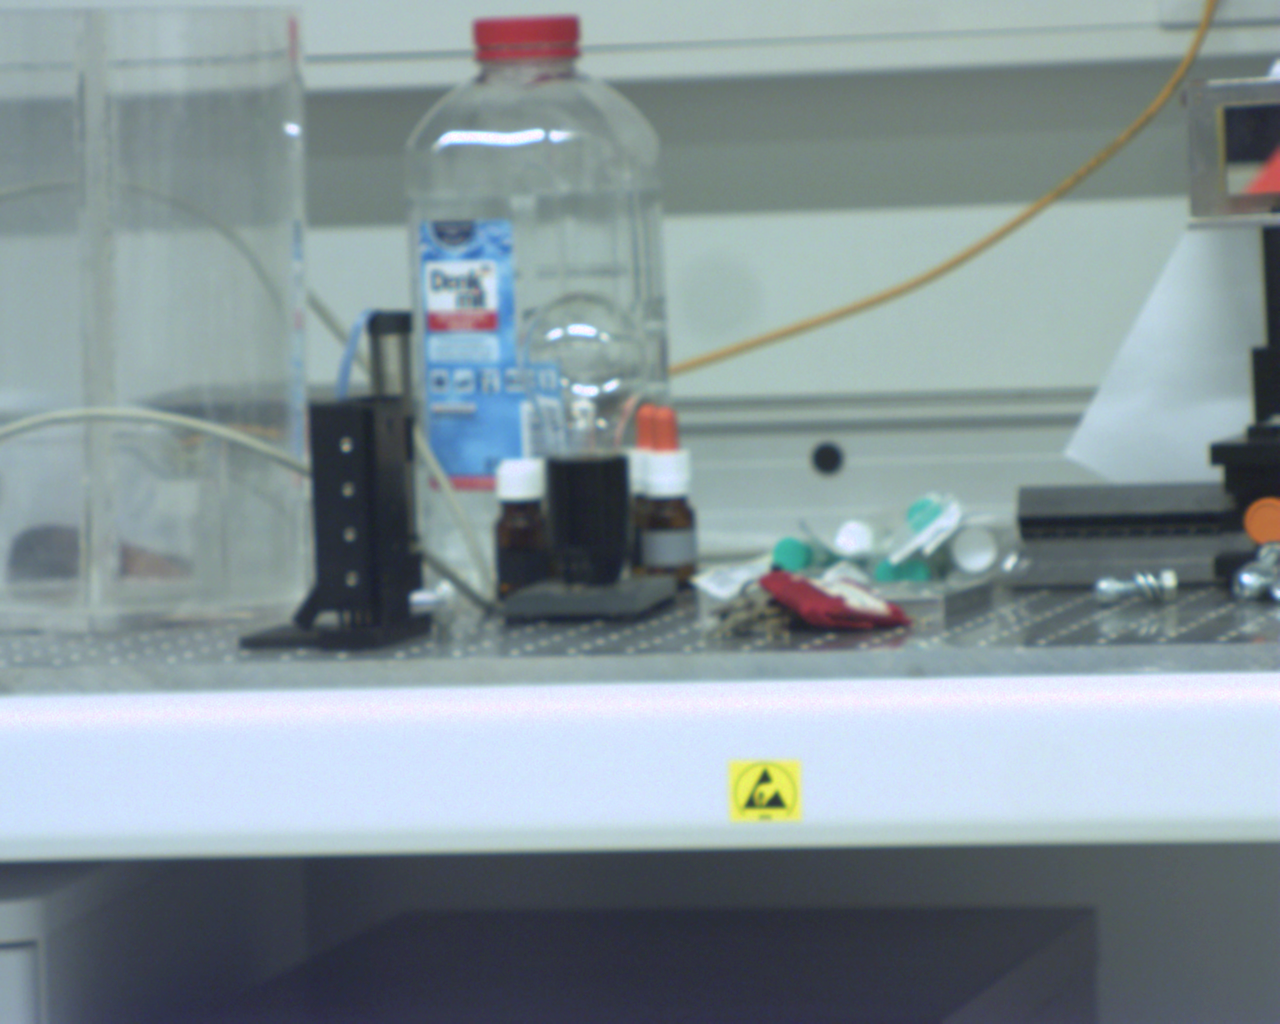
\includegraphics[width=48mm]{./Bildg_Messtechnik_Lab/Autofokus/images/image_02_0.png}\\
(a) $1.5mm$ & (b) $1.75mm$ & (c) $2.0mm$\\[6pt]
 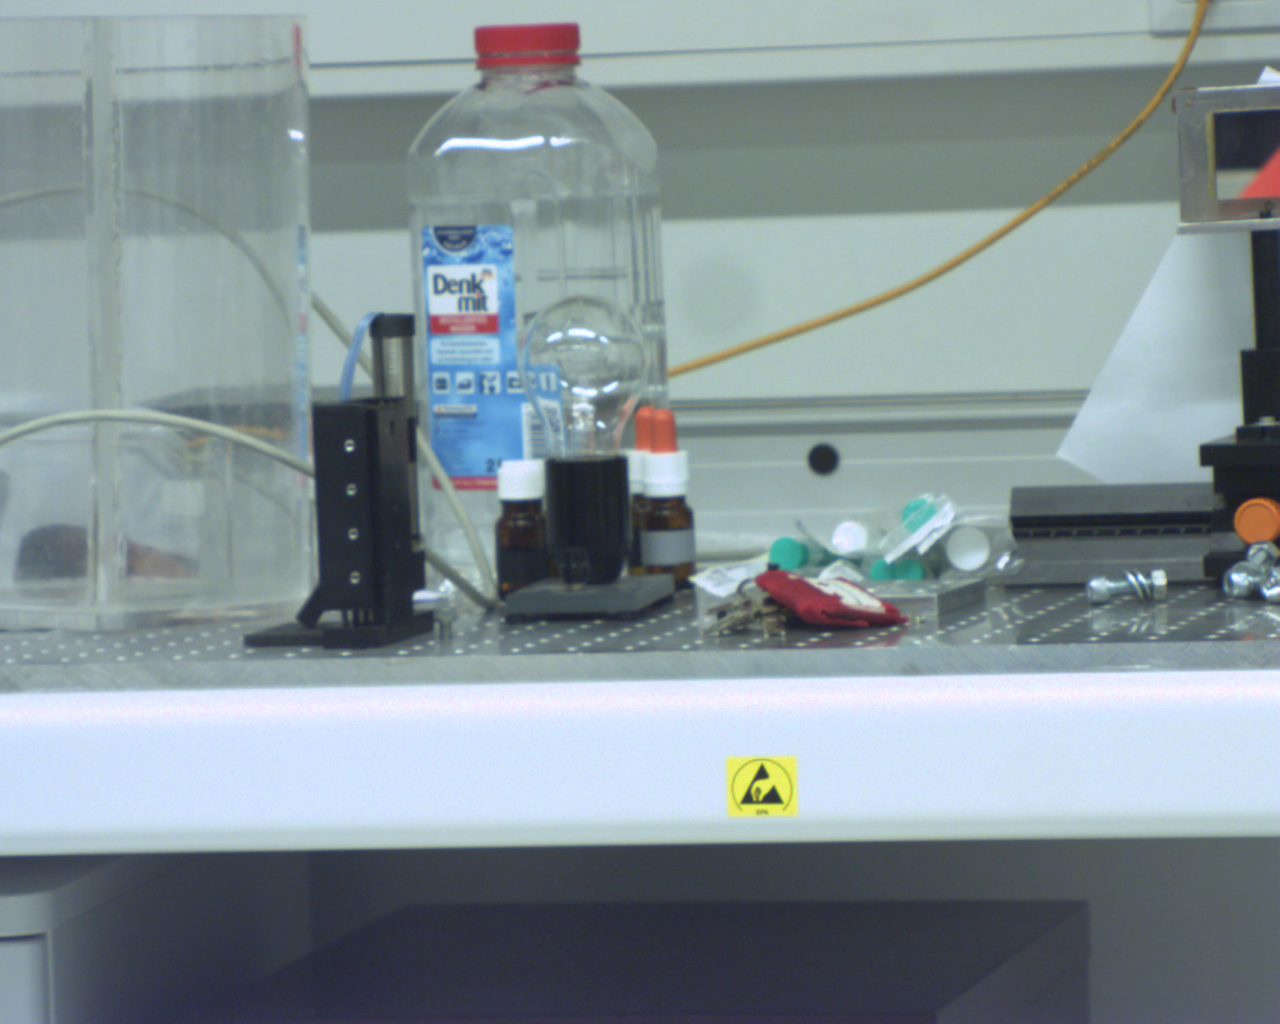
\includegraphics[width=48mm]{./Bildg_Messtechnik_Lab/Autofokus/images/image_02_5.png} & 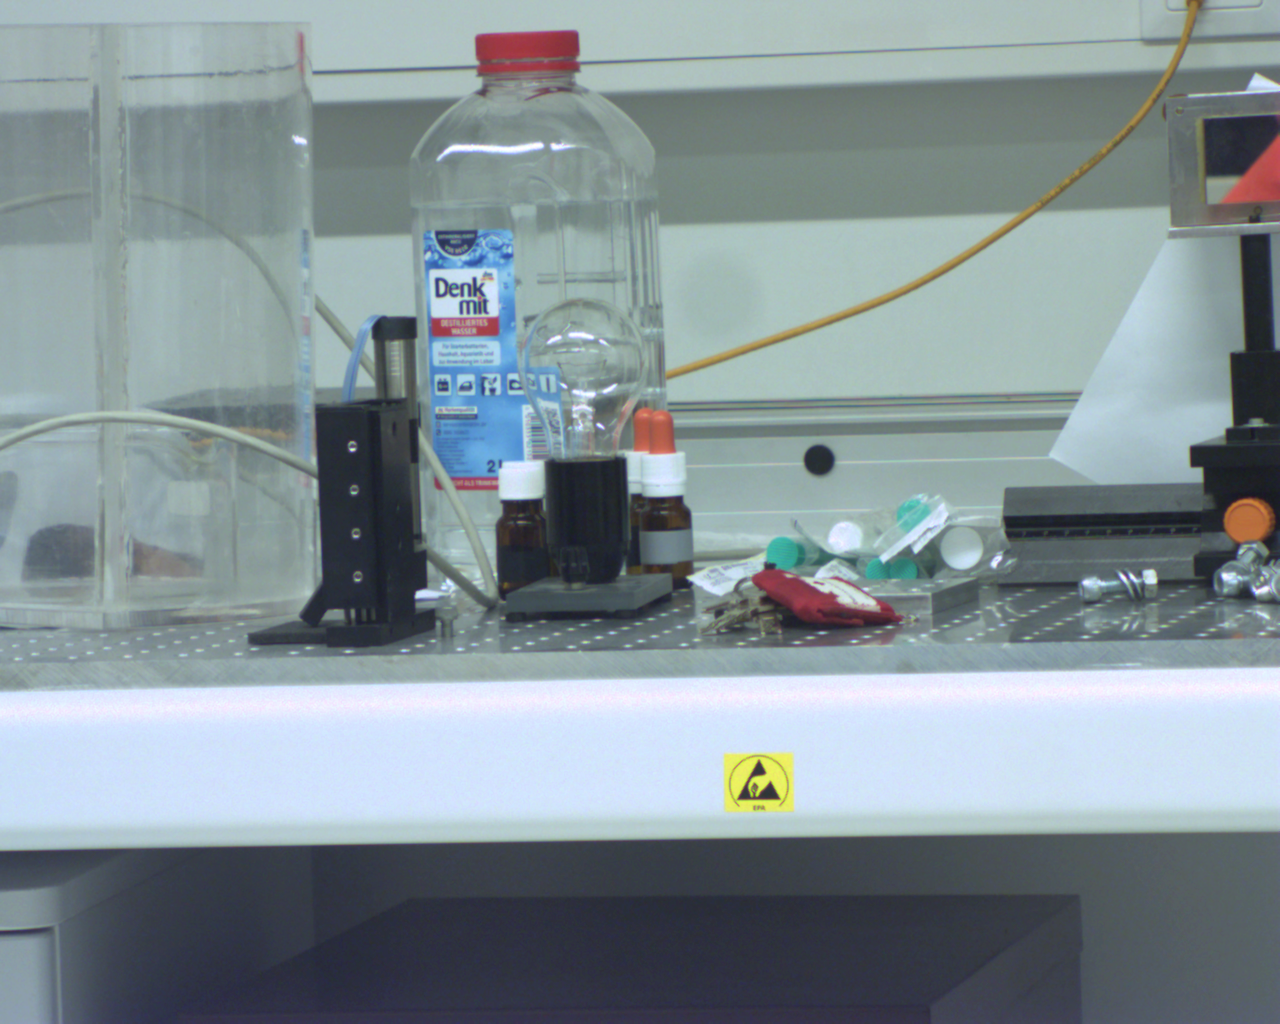
\includegraphics[width=48mm]{./Bildg_Messtechnik_Lab/Autofokus/images/image_03.png} & 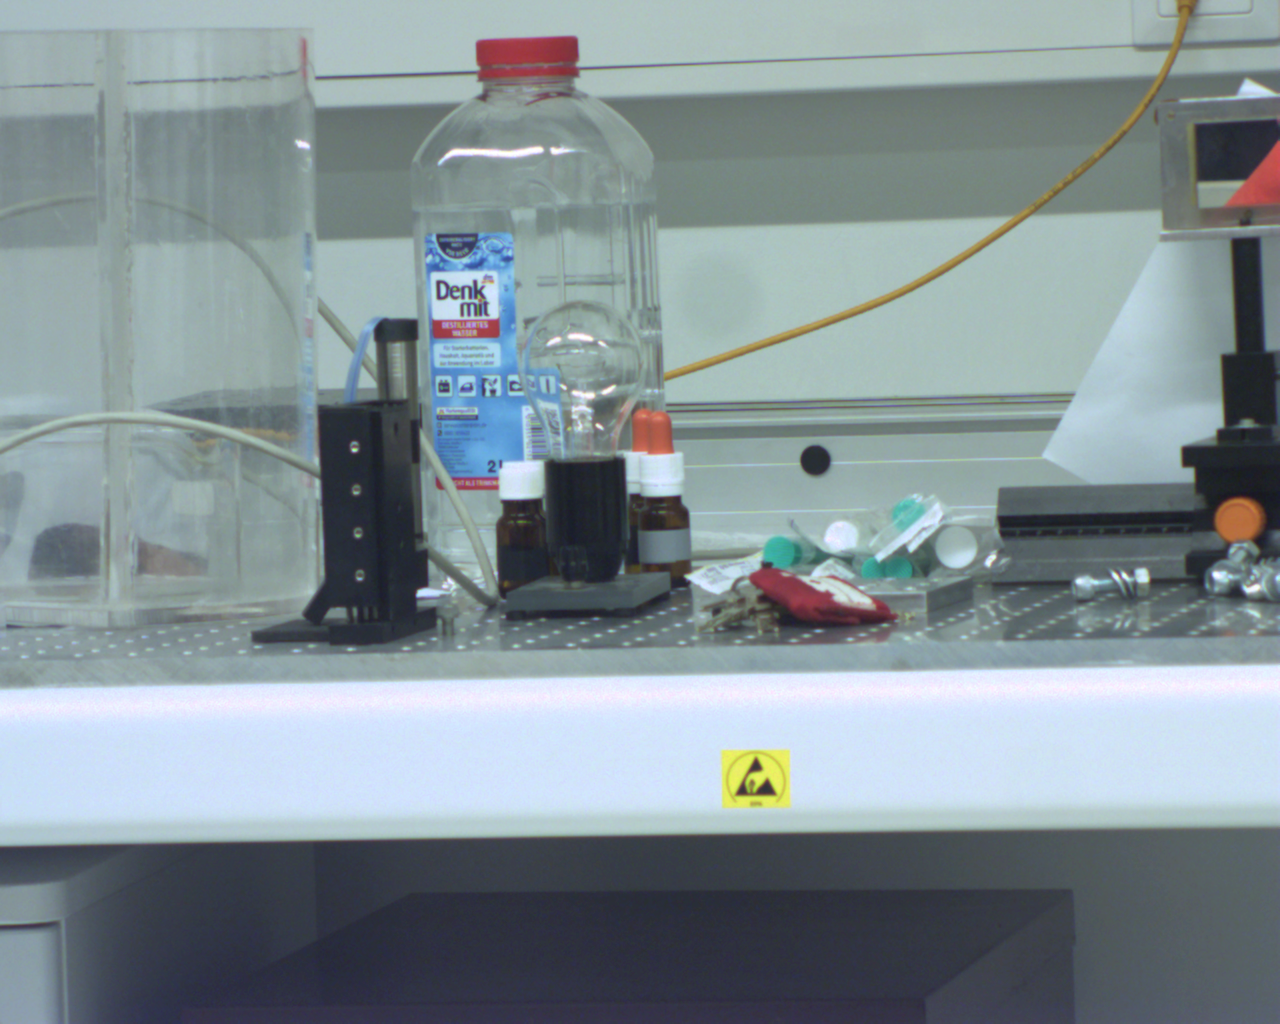
\includegraphics[width=48mm]{./Bildg_Messtechnik_Lab/Autofokus/images/image_04.png}\\
(d) $2.5mm$& (e) $3.0mm$ & (f) $4.0mm$\\[6pt]
 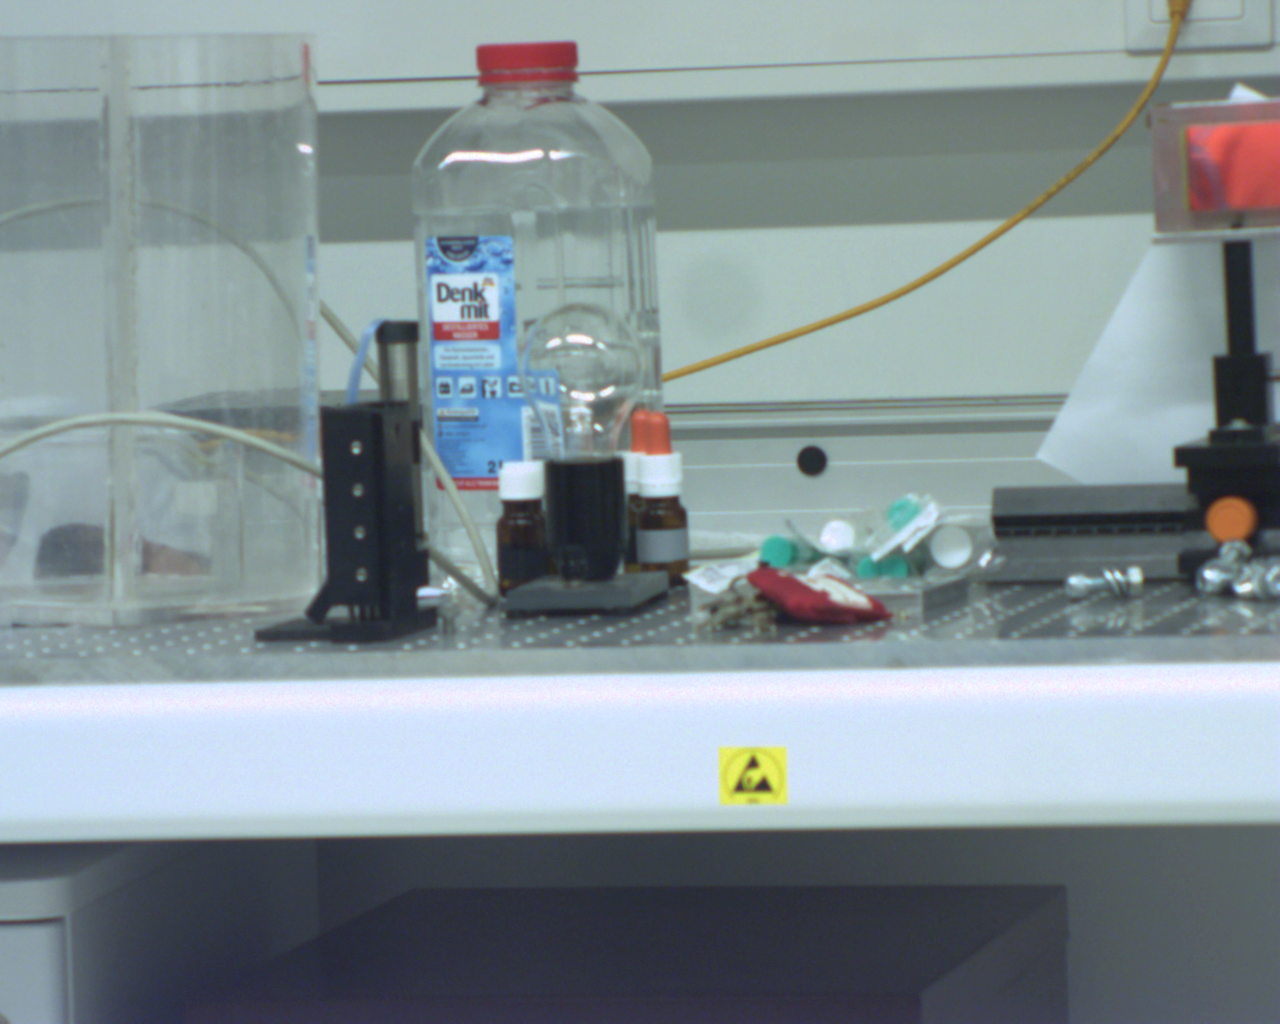
\includegraphics[width=48mm]{./Bildg_Messtechnik_Lab/Autofokus/images/image_05.png} & 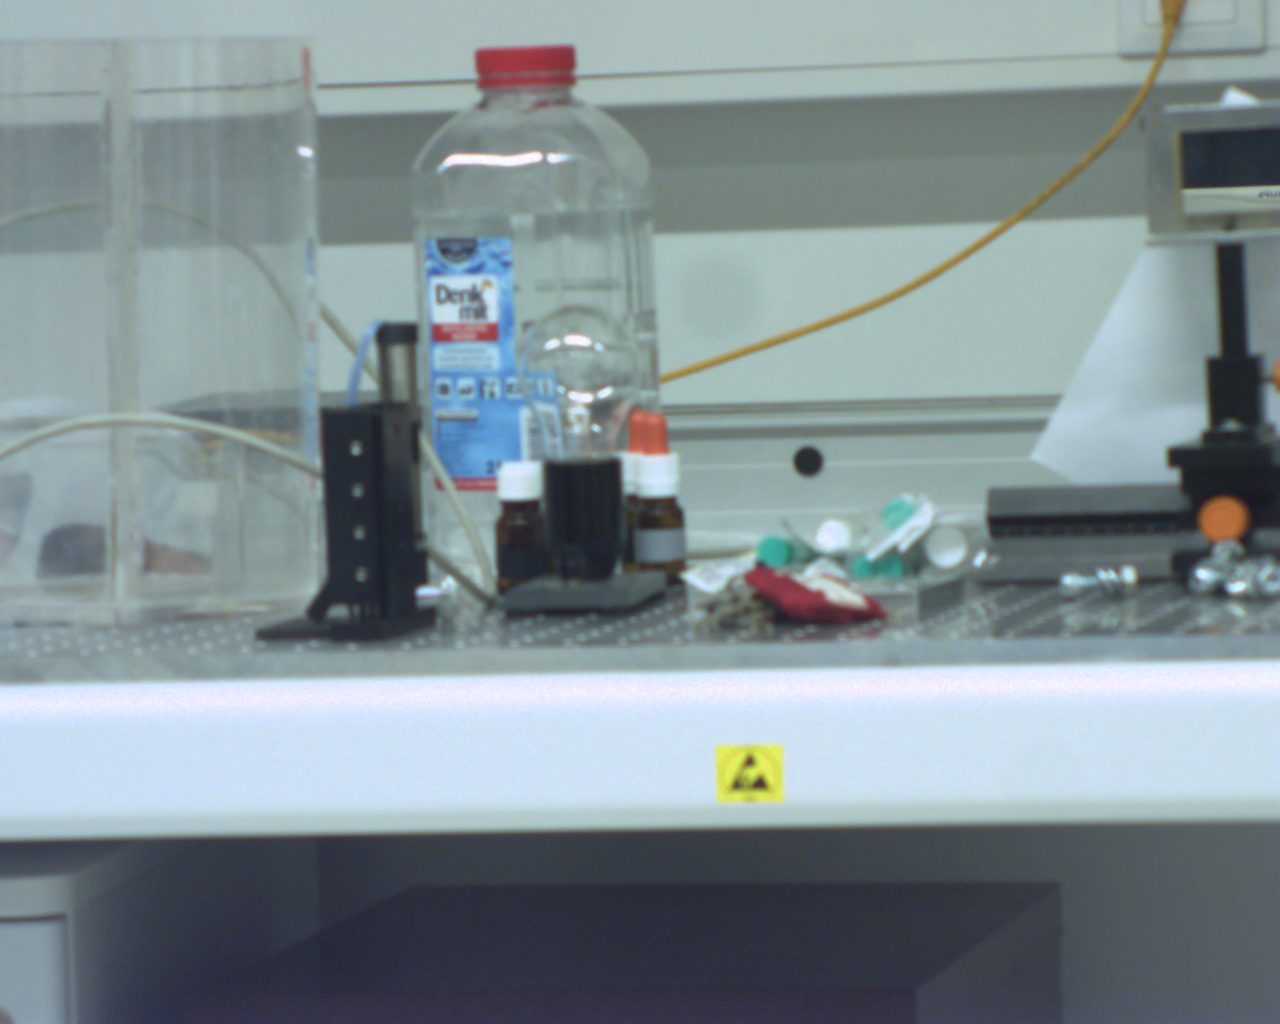
\includegraphics[width=48mm]{./Bildg_Messtechnik_Lab/Autofokus/images/image_07_5.png} & 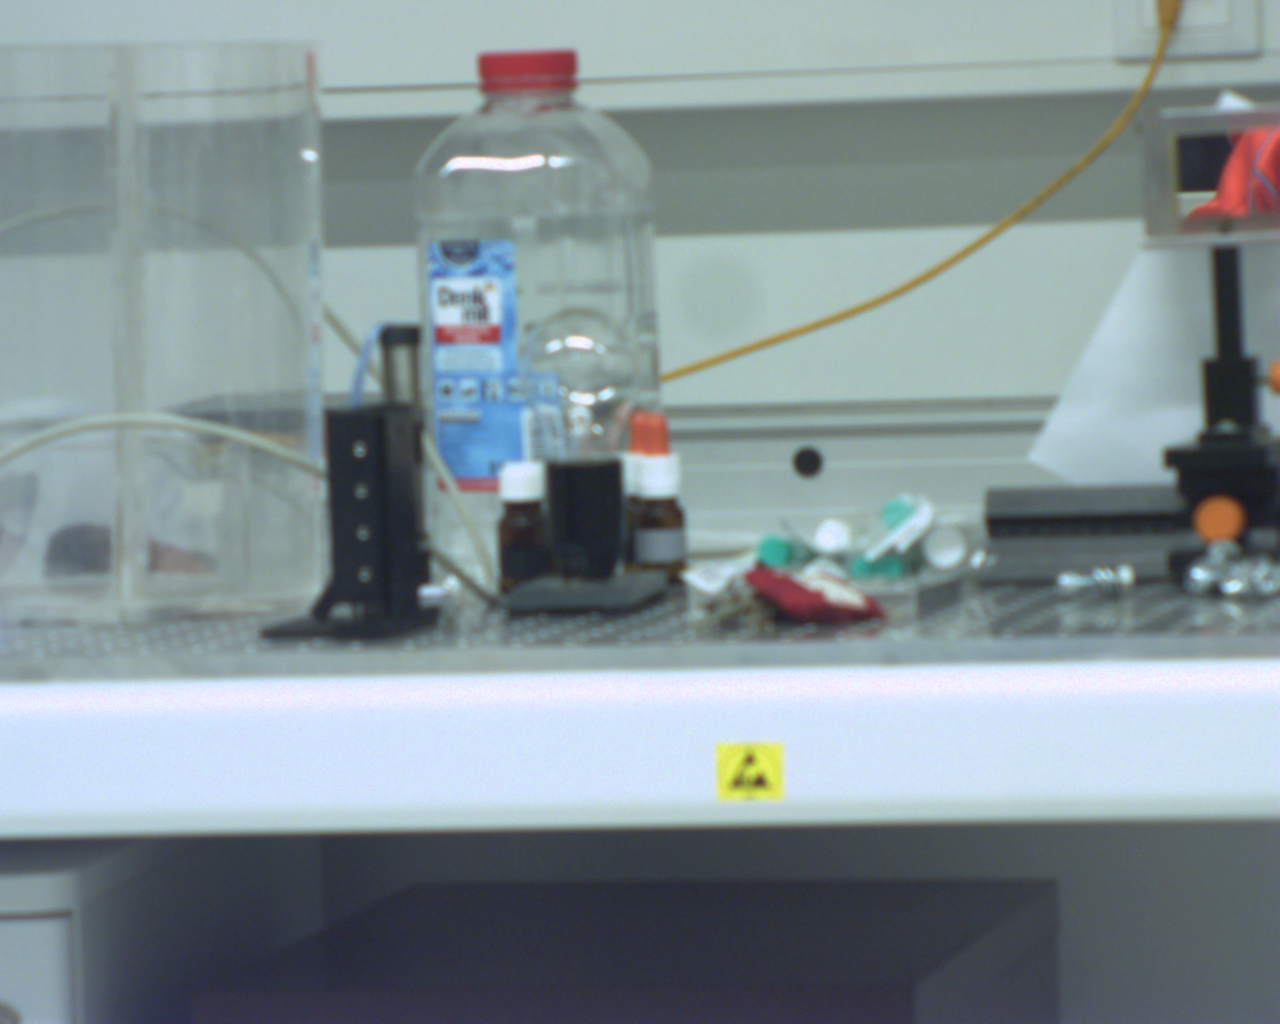
\includegraphics[width=48mm]{./Bildg_Messtechnik_Lab/Autofokus/images/image_10.png}\\
(g) $5.0mm$ & (h) $7.5mm$ & (i) $10mm$\\[6pt]
 \multicolumn{3}{c}{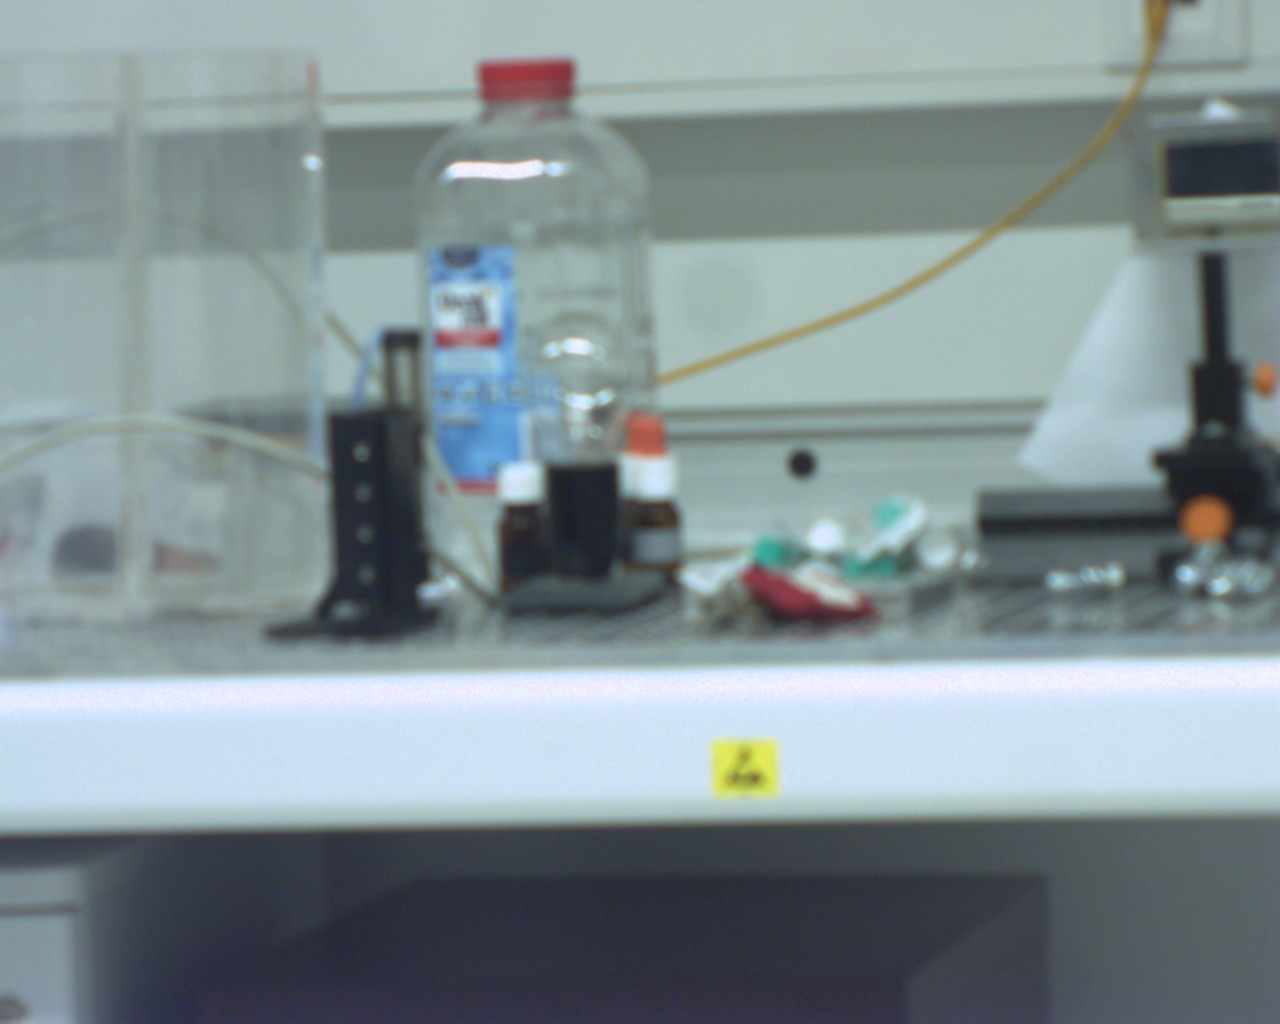
\includegraphics[width=48mm]{./Bildg_Messtechnik_Lab/Autofokus/images/image_inf.png}} \\[6pt]
 \multicolumn{3}{c}{(j) $\rightarrow\infty$}
\end{tabular}
\caption{All 10 taken images of the scene}
\label{fig:alltakenimages}
\end{figure}

\pagebreak

\section{Sensor Dynamics}

\subsection{Problem statement}

You are required to acquire an image of a detail on a rotating disc. Perform the following tasks:

\begin{itemize}
 \item Find a suitable acquisition setup (camera and illumination) using the provided camera. Investigate the use of different shutter modes.
 \item Use an integrating sensor and synchronise your light source and the rotating disc. Vary the parameters of your setup.
 \item Compare and discuss your results.
\end{itemize}

\subsection{Solution}

In this exercise a black and white colored disk with an embedded EMT logo is spun up using an electronic motor.
The goal is to take a photo of the EMT logo while the disk is spinning.
This is done using a LED flashlight which is triggered by a rotation sensor and synchronously flashes the disk.
Therefore the logo is perceived static because the light highlights the disk always when the logo is at the same place.

\subsubsection{Global Shutter}

A global shutter camera measures light intensity with all pixel sensors at the same point in time.
Figure \ref{fig:free_trigger_cont_light} shows the captured EMT logo on the disc using a global shutter with continuous lightning.

\begin{figure}[H]
 \centering
 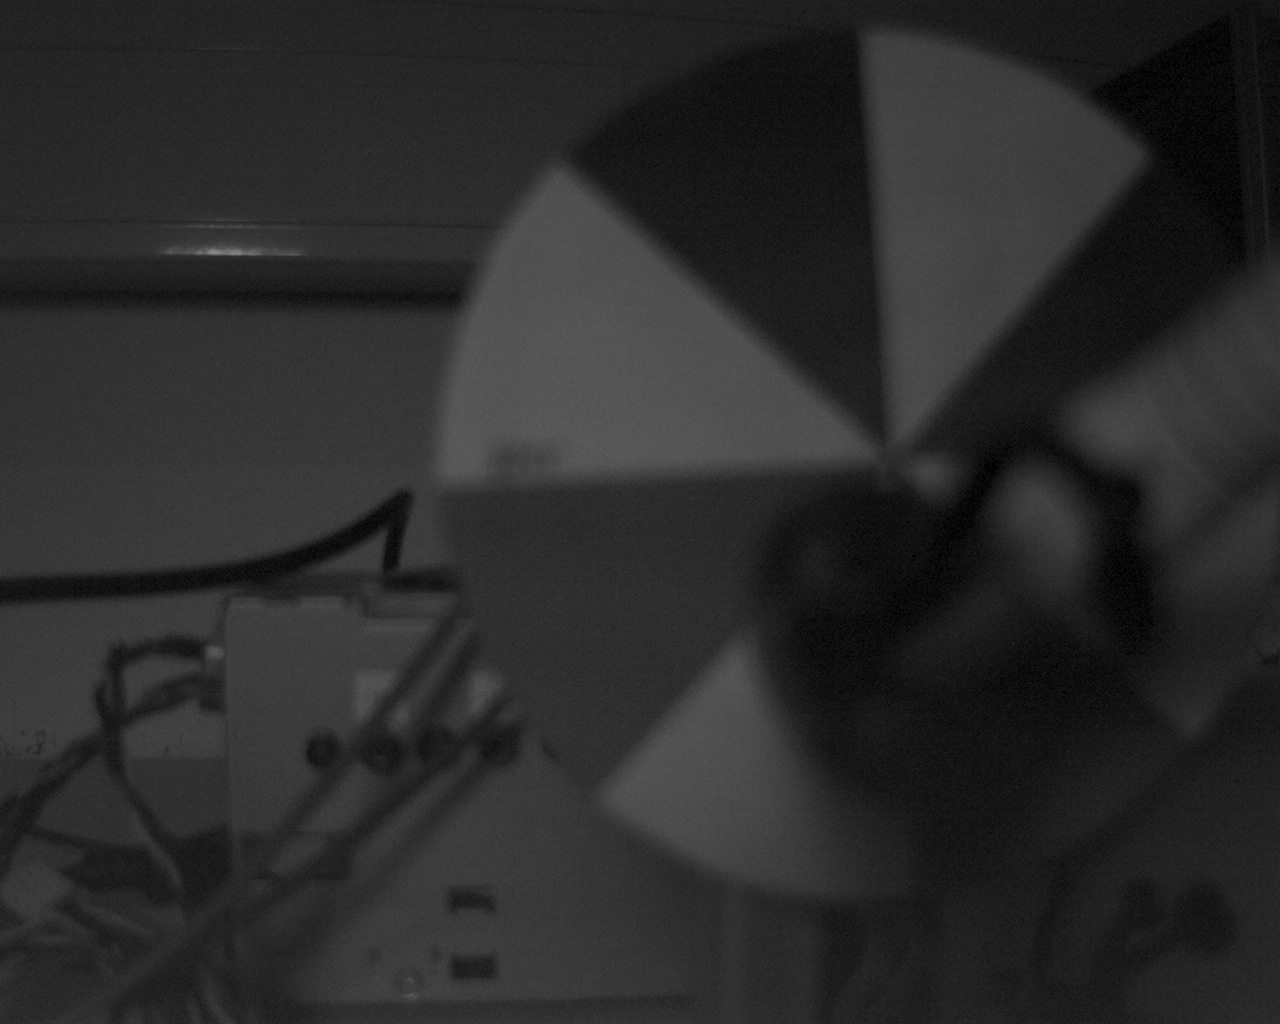
\includegraphics[width=.6\linewidth]{./Bildg_Messtechnik_Lab/SensorDynamics/free_trigger_cont_light.png}
 \caption{Free trigger with continued lightning}
 \label{fig:free_trigger_cont_light}
\end{figure}

Figure \ref{fig:triggered_9us} shows the rotating disc captured at a very high frame rate with the synchronized LED flashlight currently lighting up the logo.
The exposure time is set to only $9\mu s$.
The image is so small because we defined an area of interest which allowed the high frame rate capture over USB.

\begin{figure}[H]
 \centering
 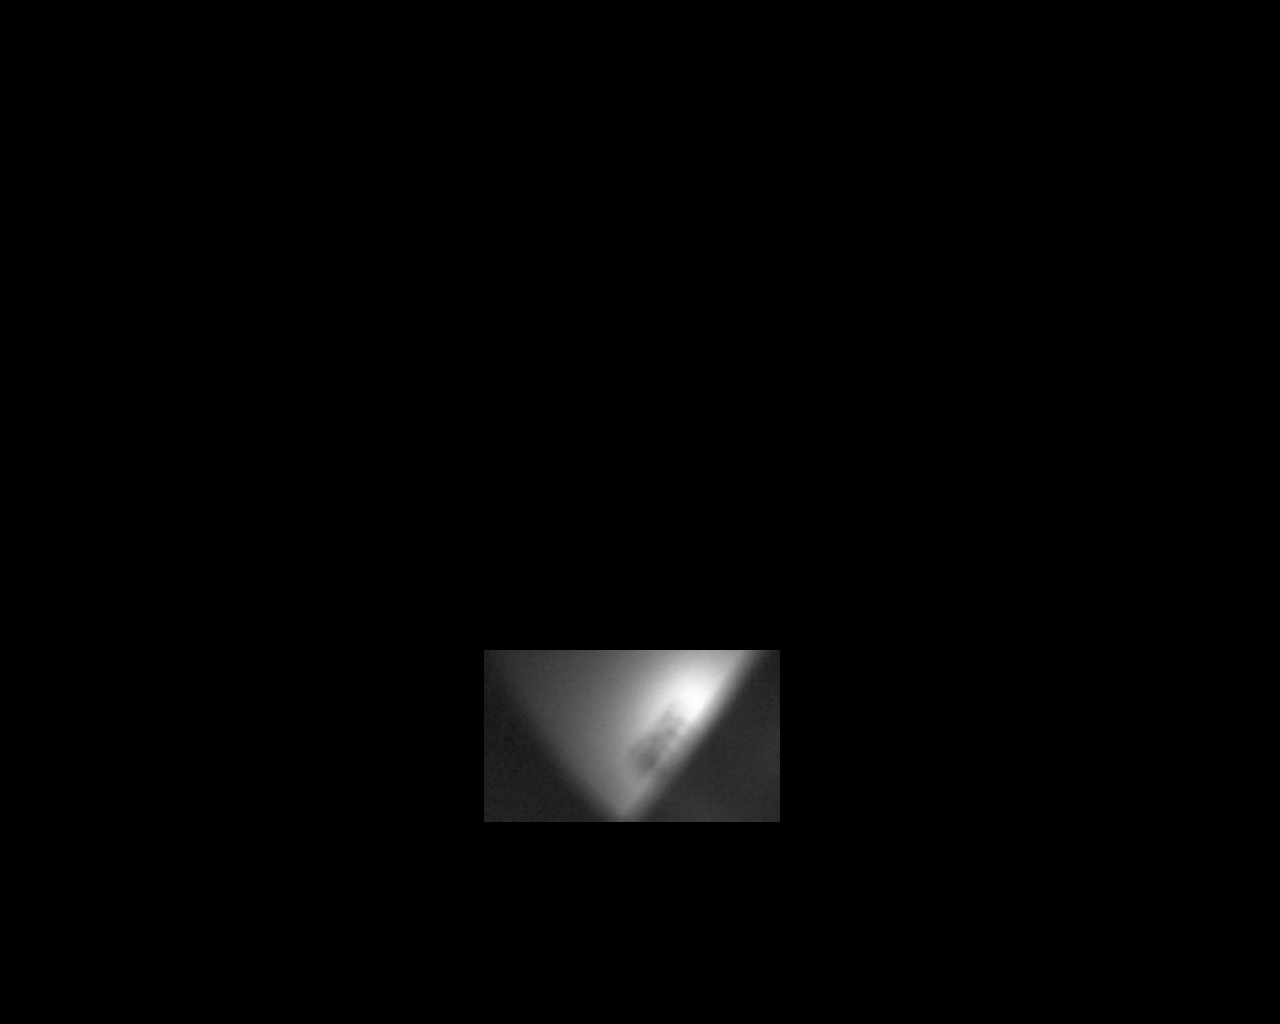
\includegraphics[width=.6\linewidth]{./Bildg_Messtechnik_Lab/SensorDynamics/triggered_9us.png}
 \caption{synchronously triggered light with $9\mu s$ exposure time}
 \label{fig:triggered_9us}
\end{figure}

Figure \ref{fig:triggered_light_189ms_exp} shows a similar capture of the EMT logo with a synchronous triggered flashlight but with a much longer exposure time of $18.9ms$.

\begin{figure}[H]
 \centering
 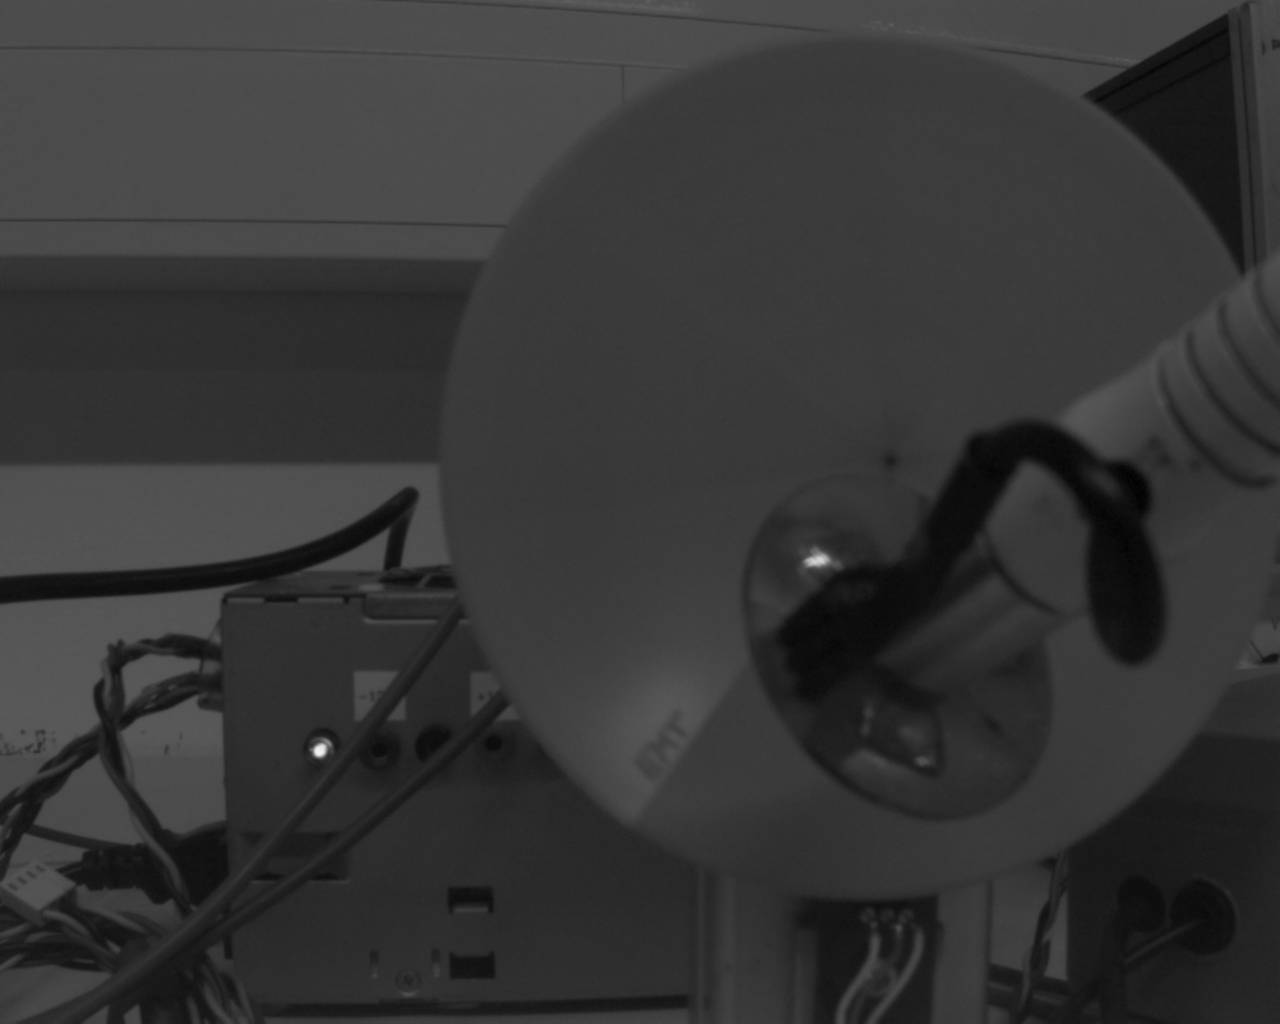
\includegraphics[width=.6\linewidth]{./Bildg_Messtechnik_Lab/SensorDynamics/triggered_light_18_9ms_exp.png}
 \caption{Triggered light with $18.9ms$ exposure time}
 \label{fig:triggered_light_189ms_exp}
\end{figure}

\subsubsection{Rolling Shutter}

A rolling shutter camera measures light intensity line by line.
This can cause certain artefacts when capturing fast moving objects as dominantly seen in Figure \ref{fig:rolling_shuter_cont_light}.

\begin{figure}[H]
 \centering
 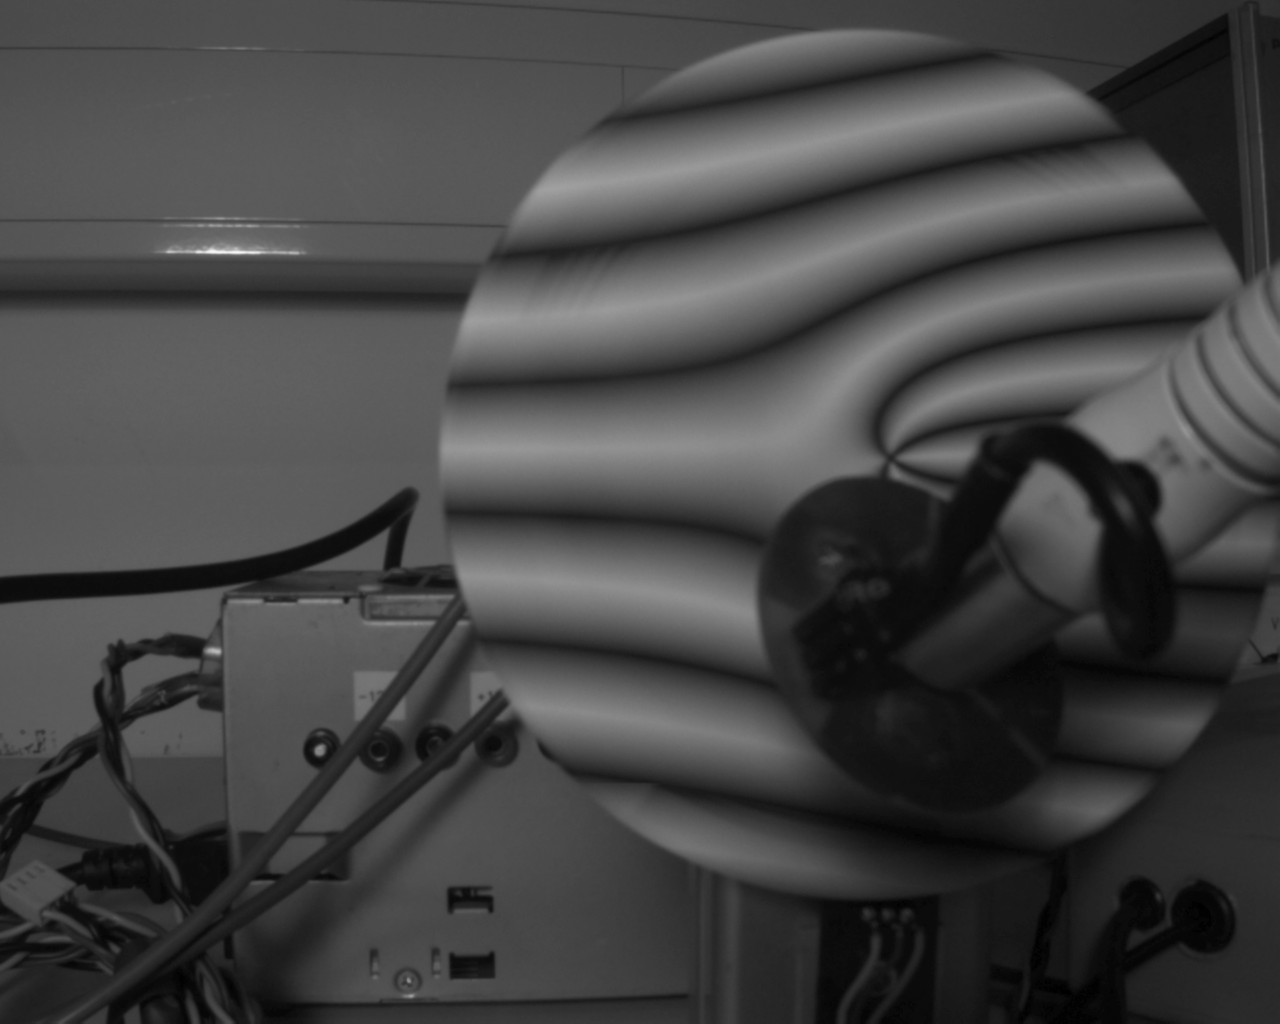
\includegraphics[width=.6\linewidth]{./Bildg_Messtechnik_Lab/SensorDynamics/rolling_shuter_cont_light.png}
 \caption{Rolling shutter with continuous lightning}
 \label{fig:rolling_shuter_cont_light}
\end{figure}

Figure \ref{fig:triggered_light_rolling_shutter} shows a rolling shutter when using triggered light to capture the EMT logo.

\begin{figure}[H]
 \centering
 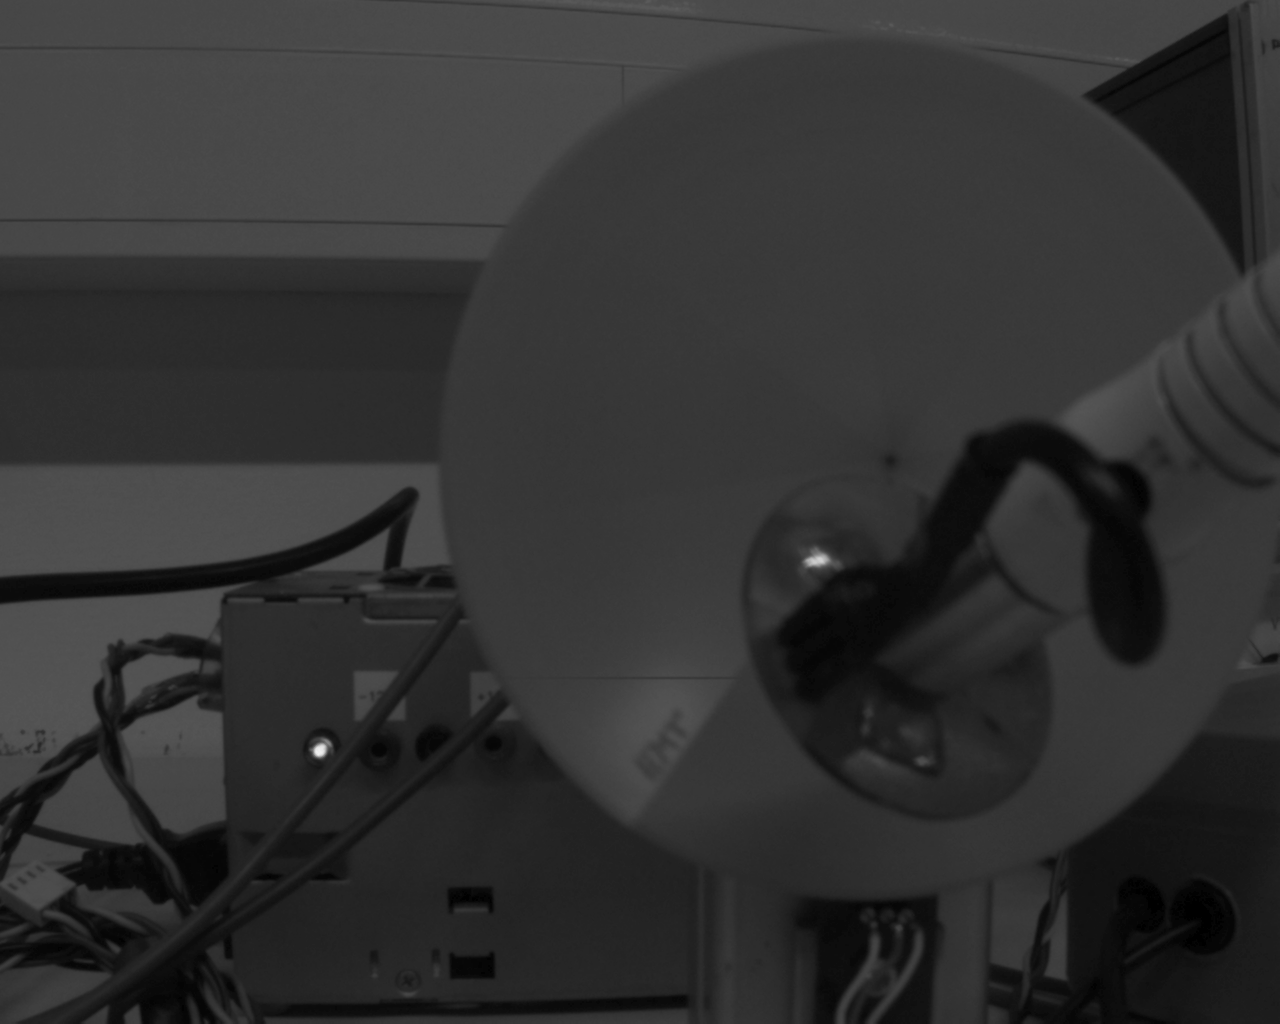
\includegraphics[width=.6\linewidth]{./Bildg_Messtechnik_Lab/SensorDynamics/triggered_light_rolling_shutter.png}
 \caption{Triggered light with $18.9ms$ exposure time}
 \label{fig:triggered_light_rolling_shutter}
\end{figure}


\pagebreak
\section{Perspective Invariants}

\subsection{Problem statement}

Investigate the Cross Ratio $(CR)$ of four co-linear points $A, B, C,$ and $D$ as given by

\begin{equation}
 CR_{A,B,C,D} = \frac{\overline{AC}}{\overline{BC}} : \frac{\overline{AD}}{\overline{BD}}
 \label{eq:cross_ratio}
\end{equation}

The $CR$ is invariant under perspective projections. Use a CR-Target to acquire $N = 10$ images under varying
viewing conditions and perform the following tasks:

\begin{itemize}
 \item Extract the required points $A, B, C,$ and $D$ using a corner detector.
 \item Complete the MATLAB function \texttt{CrossRatio.m} to measure the $CR$.
 \item Determine the histogram, mean-value, and standard deviation of the $CR$ over all images.
 \item Visualise and discuss your results.
\end{itemize}


\subsection{Solution}

In this exercise we take photos of a $CR$-target which contains four points that have a certain distance to each other.
The points are prepared to easily be detected by a \lstinline{cornerMark} function which is given by the framework.
Two different cameras with focal length of $4.3mm$ and $12.5mm$ were used.
\\
The claim to verify is that formula \ref{eq:cross_ratio} is independent of the perspective the picture is taken from as well as independent of the used focal length.

\subsubsection{Measuring by hand}

The first step we took to verify this claim is to measure the distance of the points on the targets using a ruler and calculate the ideal values which should be reached by the taken images.
Formula \ref{eq:measure_by_hand} calculates the ideal Cross Ratio.

\begin{minipage}{0.48\textwidth}
  $$\overline{AB} = 42mm$$
  $$\overline{BC} = 82mm$$
  $$\overline{CD} = 123mm$$
\end{minipage}
\begin{minipage}{0.48\textwidth}
  $$\overline{AC} = 123mm$$
  $$\overline{BD} = 205mm$$
  $$\overline{AD} = 246mm$$
\end{minipage}

\hspace{0.5mm}

\begin{equation}
 CR_{A,B,C,D} = \frac{\overline{AC}}{\overline{BC}} : \frac{\overline{AD}}{\overline{BD}} = \frac{123mm}{82mm} : \frac{246mm}{205mm} = 1.25
 \label{eq:measure_by_hand}
\end{equation}

\subsubsection{Measuring using the cornerMark Matlab algorithm}

After this step we took $N = 5$ (Should be enough to calculate a good approximation) photos of different perspectives with different focal lengths.
These photos can be seen in Figure \ref{fig:cornermark_images}.
The top row of the target was chosen in this case.
Listing \ref{lst:main_cross_ratio} shows how the calculation was achieved.
Line $23$ iterates over all images.
Using the \lstinline{markCorners(...)} function given by the framework the points can be chosen via a graphical user interface.
If one point is set by the GUI the markCorners function tries to find the middle of the square.
Then, the $CR$ is calculated using the \lstinline{CrossRatio(...)} function of which the implementation can be seen in Listing \ref{lst:crossratio}.
Finally the average and the standard deviation of the cross function matrix are calculated using the \lstinline{mean(...)} and \lstinline{std(...)} Matlab functions.

\lstinputlisting[label=lst:main_cross_ratio, caption=Main script]{./Bildg_Messtechnik_Lab/CrossRatio/main.m}

\lstinputlisting[label=lst:crossratio, caption=Cross Ratio function implementation]{./Bildg_Messtechnik_Lab/CrossRatio/CrossRatio.m}

Table \ref{tab:cross_ratios} shows that the results are all very close to the measured ideal value.
The first five entries of the table are the measured $CR$s of the pictures taken by the $4.3mm$ focal length camera and the five following entries represent the $CR$s of the Pictures taken by the $12.5mm$ camera.
The average result is $1.248$ with a standard deviation of $0.0013$ and is therefore only $0.002$ off of the ideally measured value which is $1.250$.
So it is save to say that the $CR$ is perspective independent.

\begin{table}[ht!]
  \centering
  \begin{tabular}{|c|c|c|c|c||c|c|c|c|c|}\hline
    1.248 & 1.247 & 1.246 & 1.246 & 1.246 & 1.248 & 1.249 & 1.249 & 1.248 & 1.248\\\hline
  \end{tabular}
  \caption{Cross ratios for $4.3mm$ and $12.5mm$ focal length}
  \label{tab:cross_ratios}
\end{table}


\begin{figure}[ht!]
\centering
\begin{tabular}{ccc}
 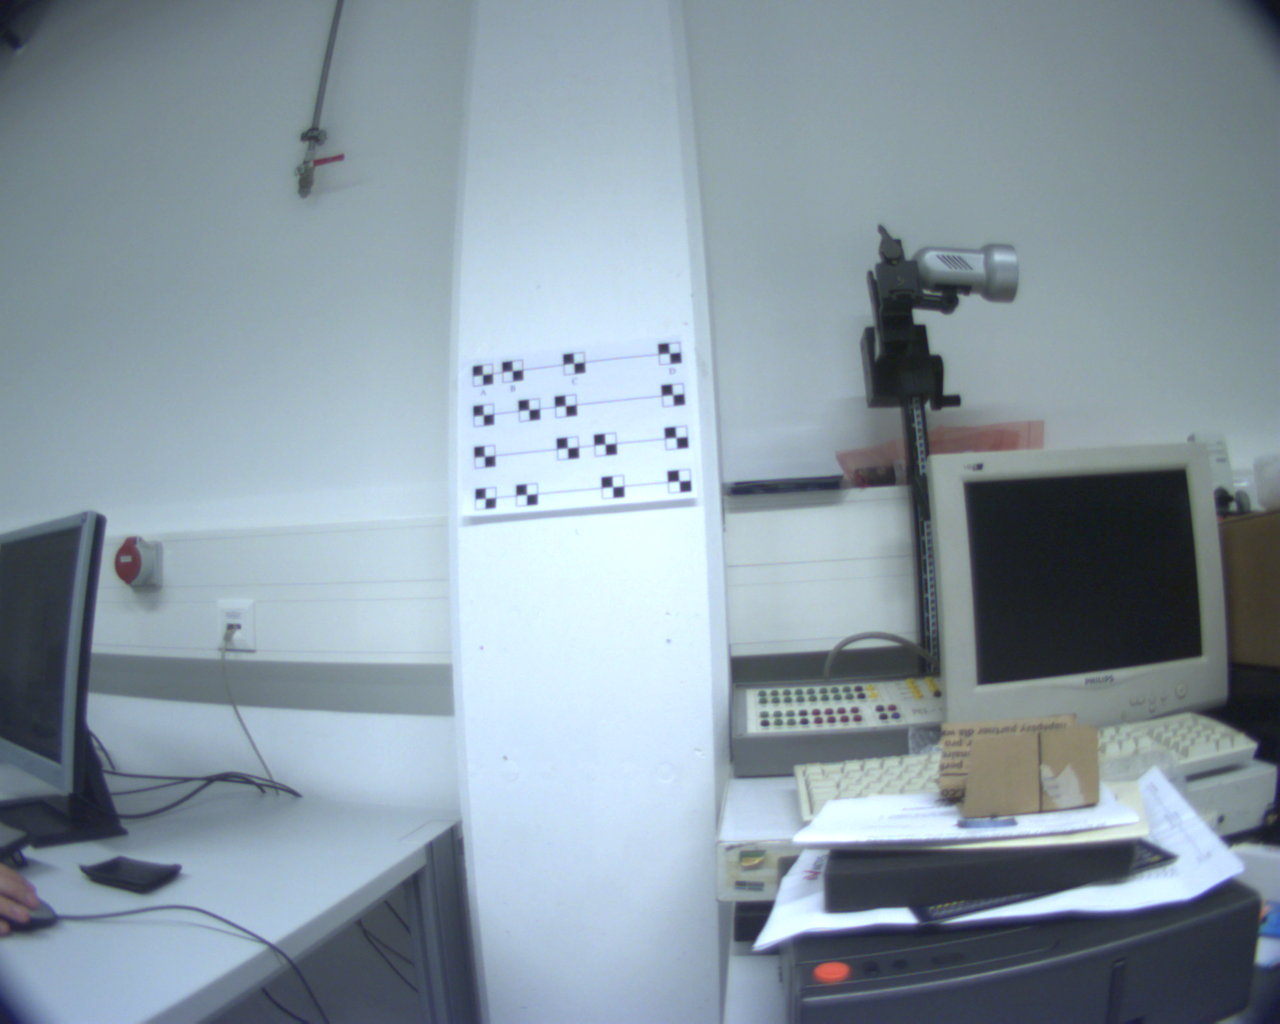
\includegraphics[width=48mm]{./Bildg_Messtechnik_Lab/CrossRatio/images/image_a1.png} & 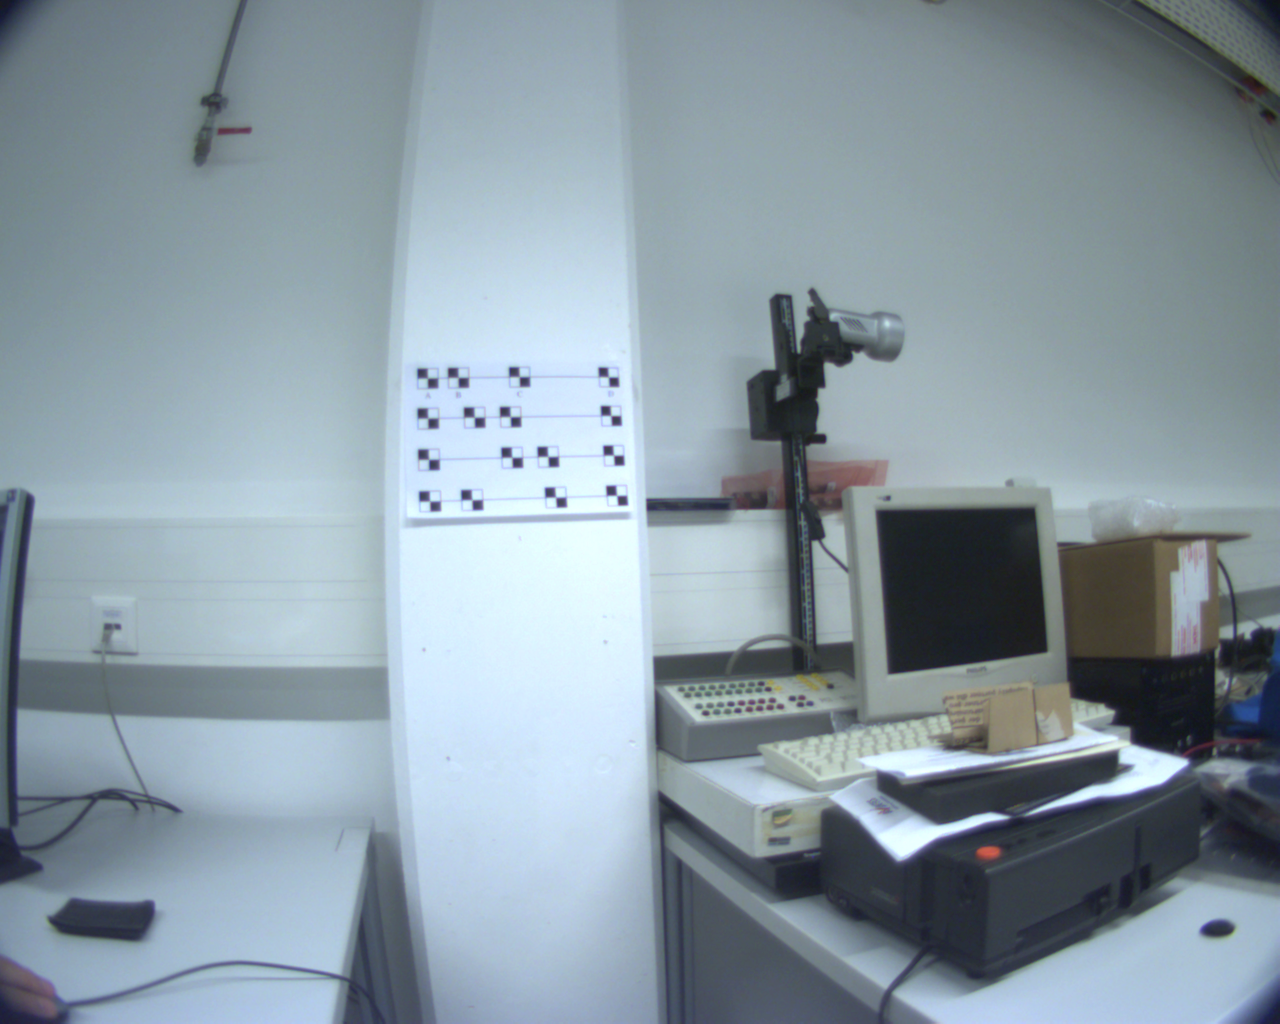
\includegraphics[width=48mm]{./Bildg_Messtechnik_Lab/CrossRatio/images/image_a2.png} & 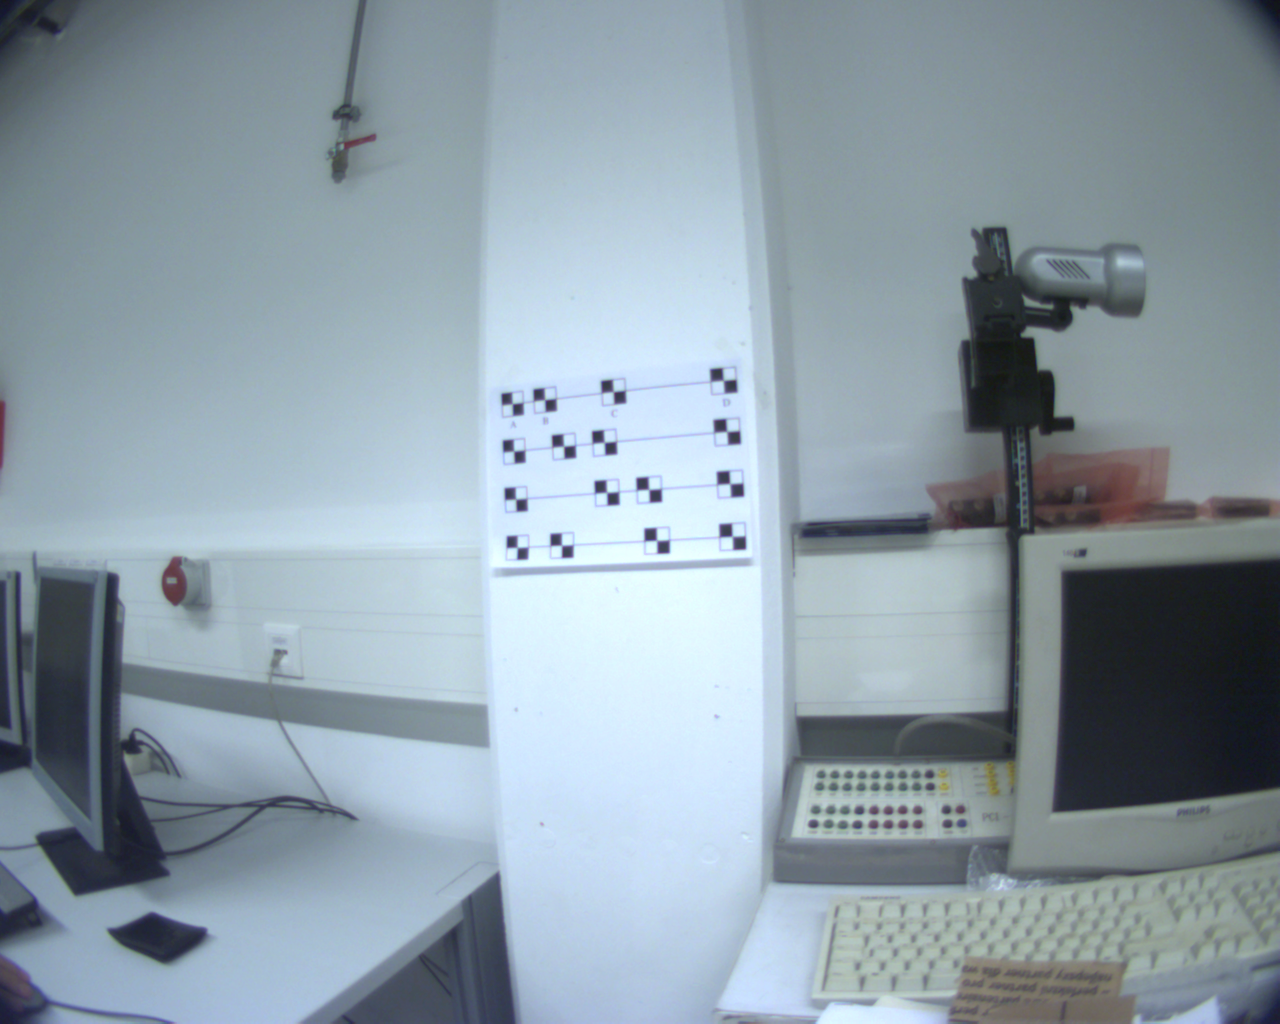
\includegraphics[width=48mm]{./Bildg_Messtechnik_Lab/CrossRatio/images/image_a3.png}\\
(a) $4.3mm$ & (b) $4.3mm$ & (c) $4.3mm$\\[6pt]
 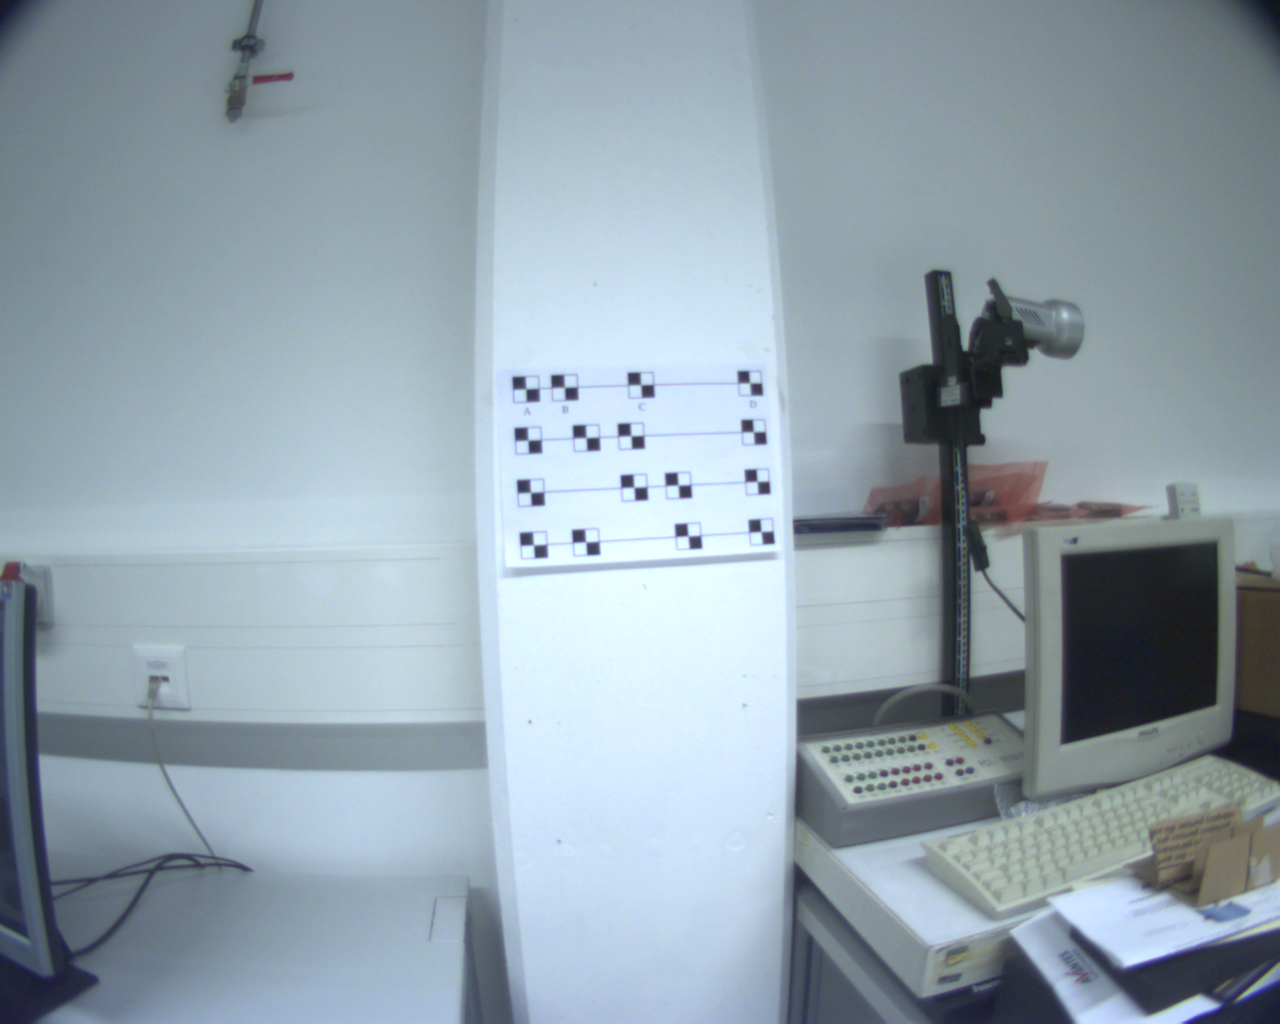
\includegraphics[width=48mm]{./Bildg_Messtechnik_Lab/CrossRatio/images/image_a4.png} & 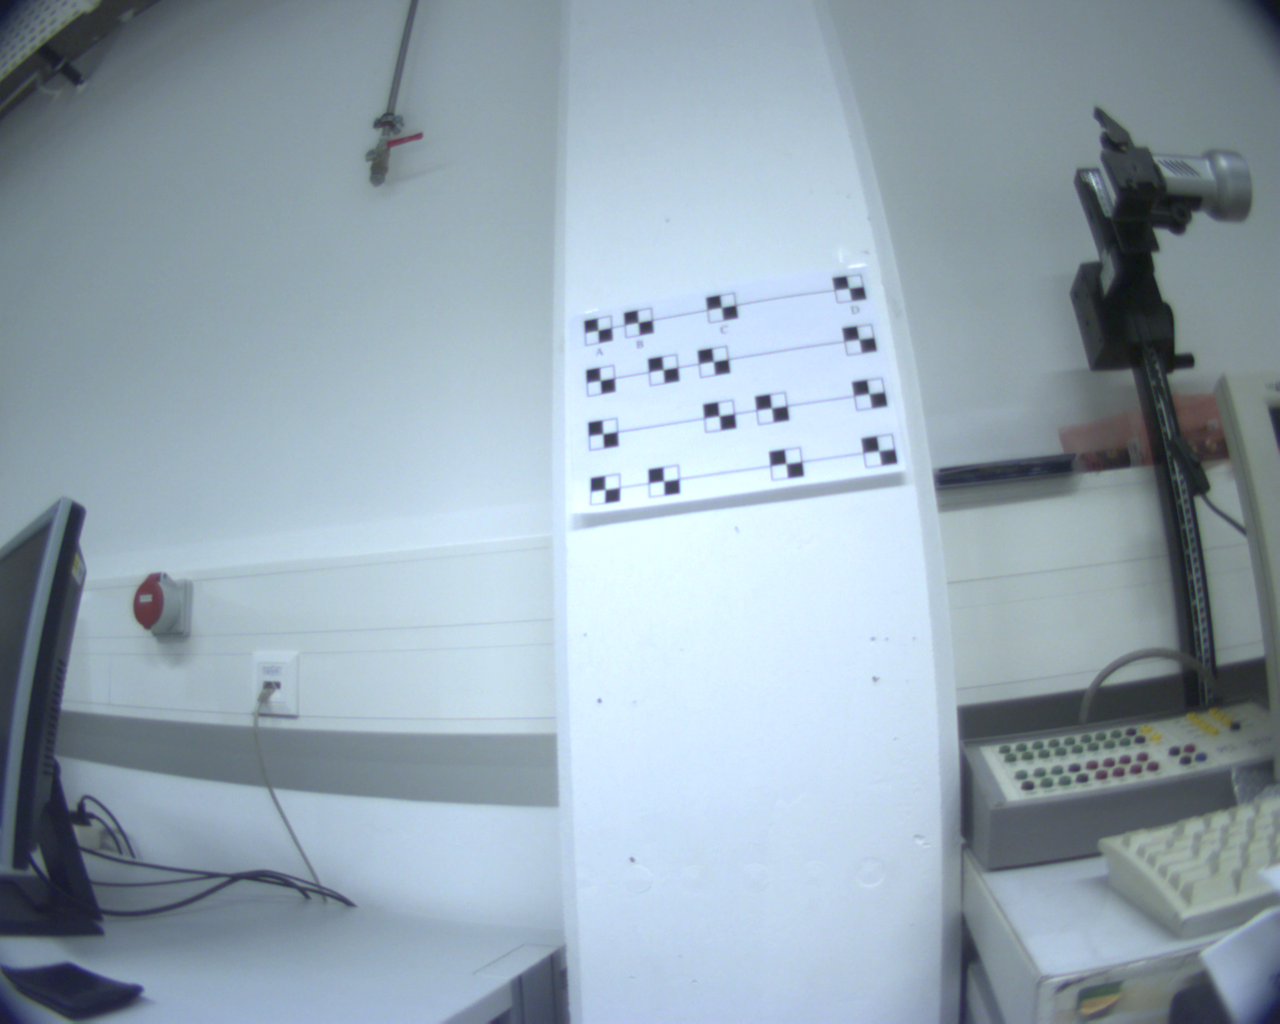
\includegraphics[width=48mm]{./Bildg_Messtechnik_Lab/CrossRatio/images/image_a5.png} & 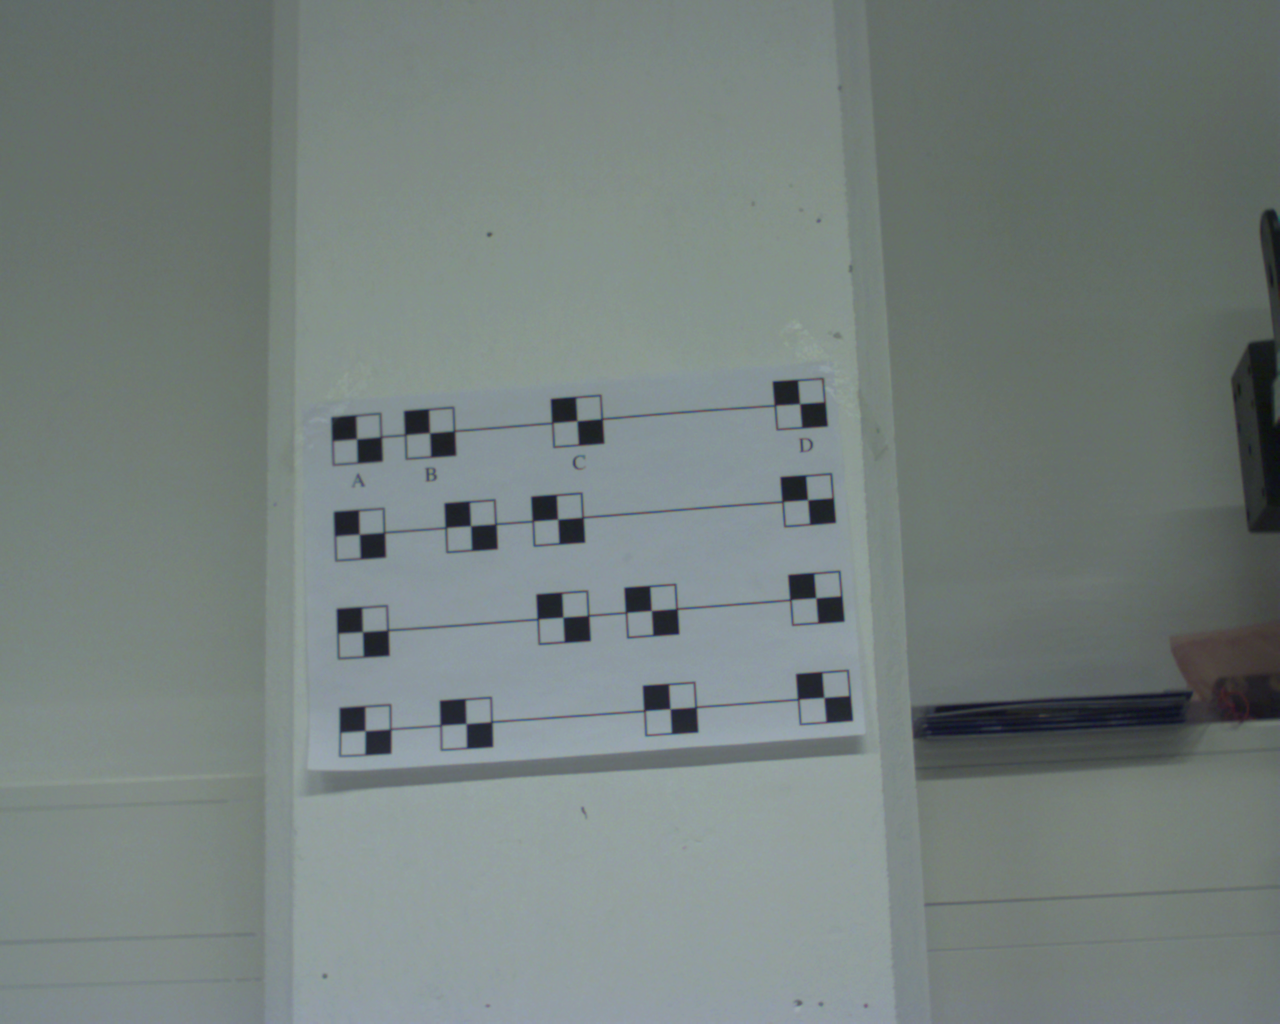
\includegraphics[width=48mm]{./Bildg_Messtechnik_Lab/CrossRatio/images/image_b1.png}\\
(d) $4.3mm$& (e) $4.3mm$ & (f) $12.5mm$\\[6pt]
 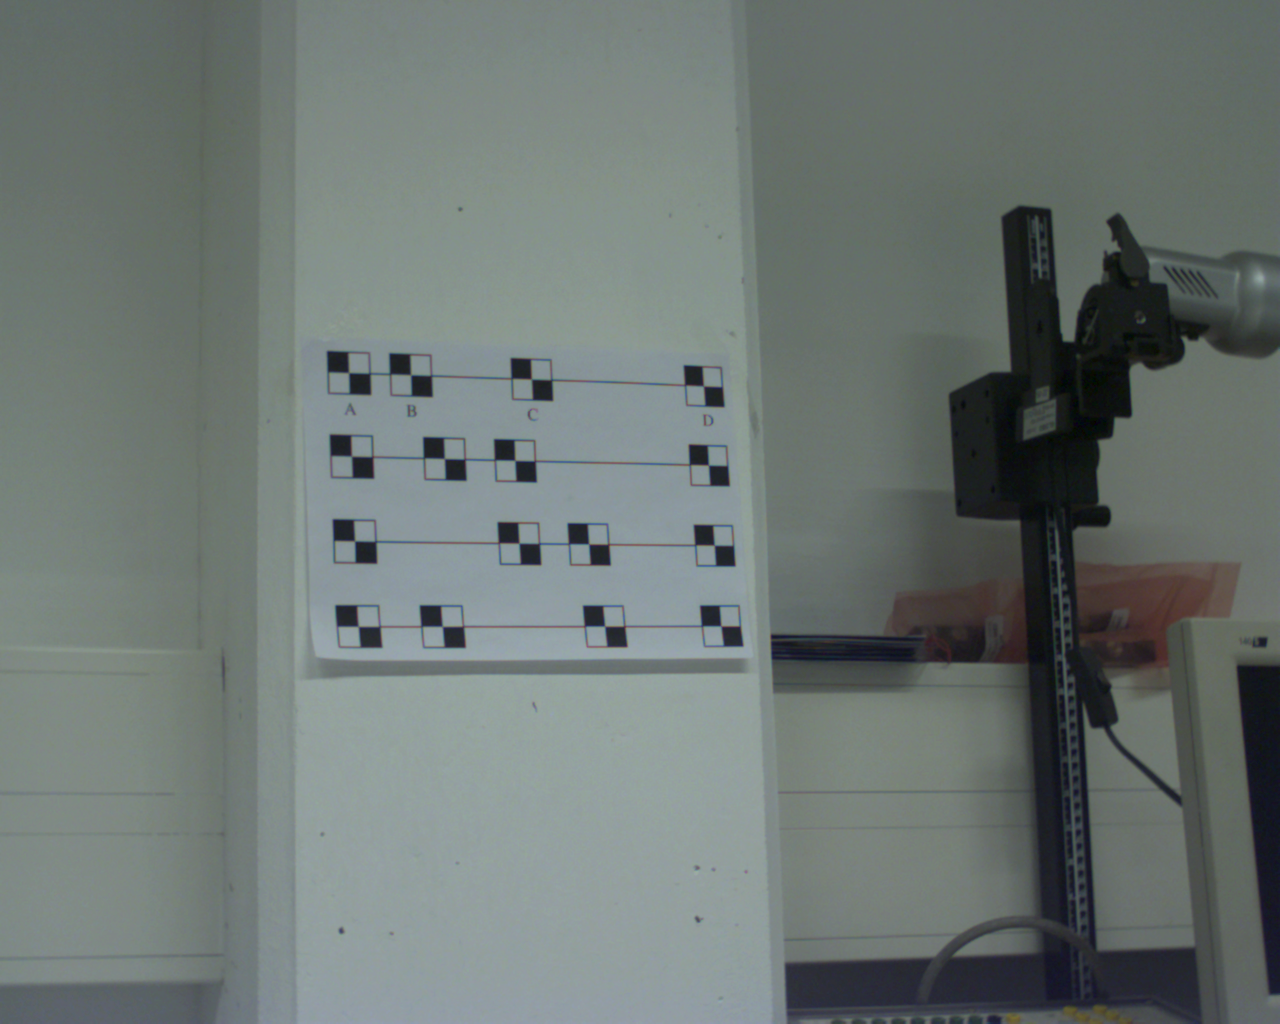
\includegraphics[width=48mm]{./Bildg_Messtechnik_Lab/CrossRatio/images/image_b2.png} & 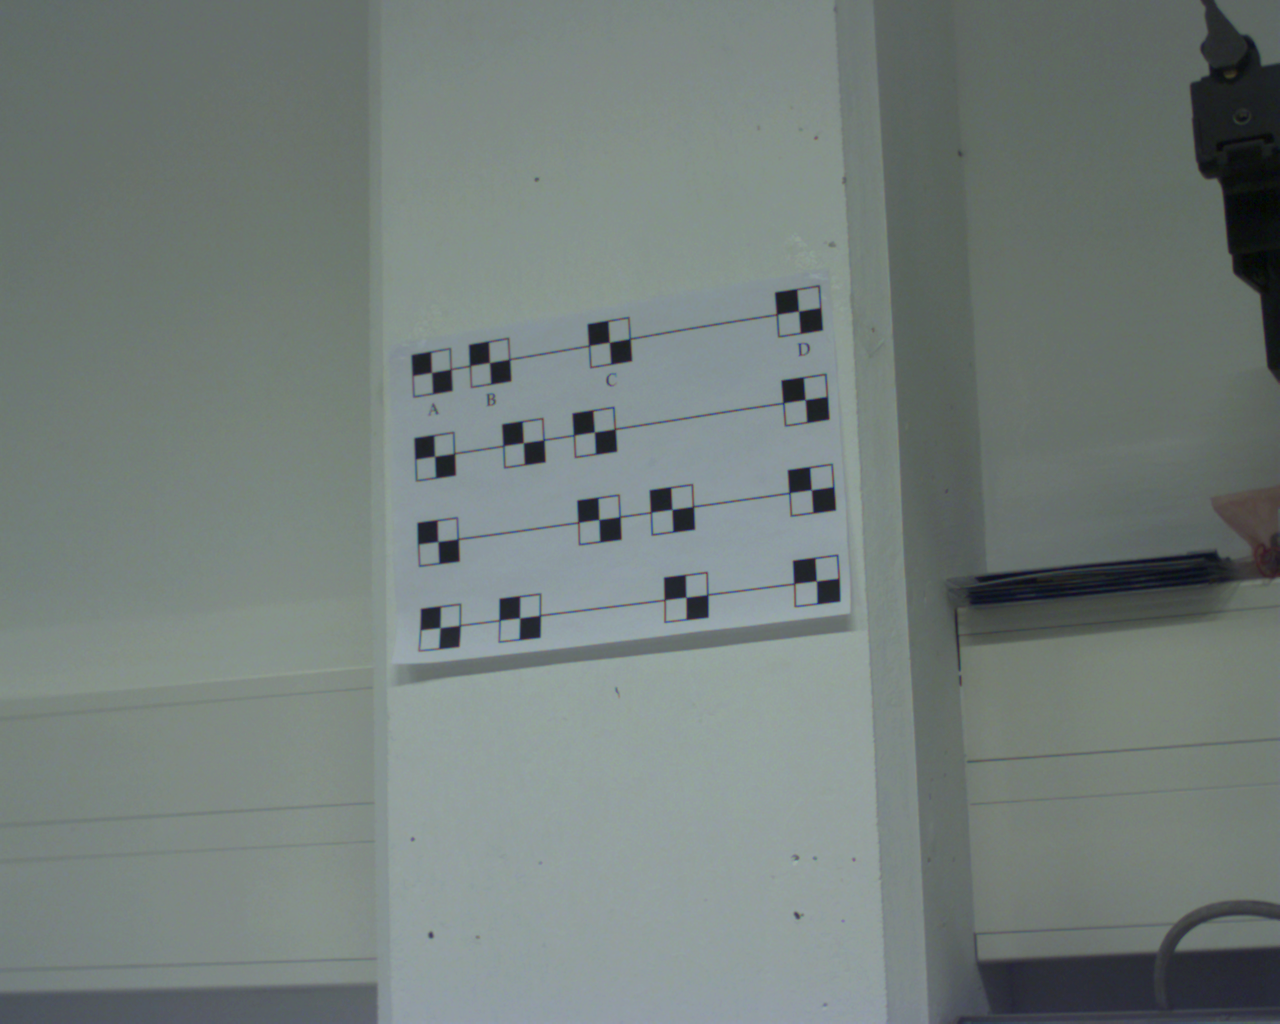
\includegraphics[width=48mm]{./Bildg_Messtechnik_Lab/CrossRatio/images/image_b3.png} & 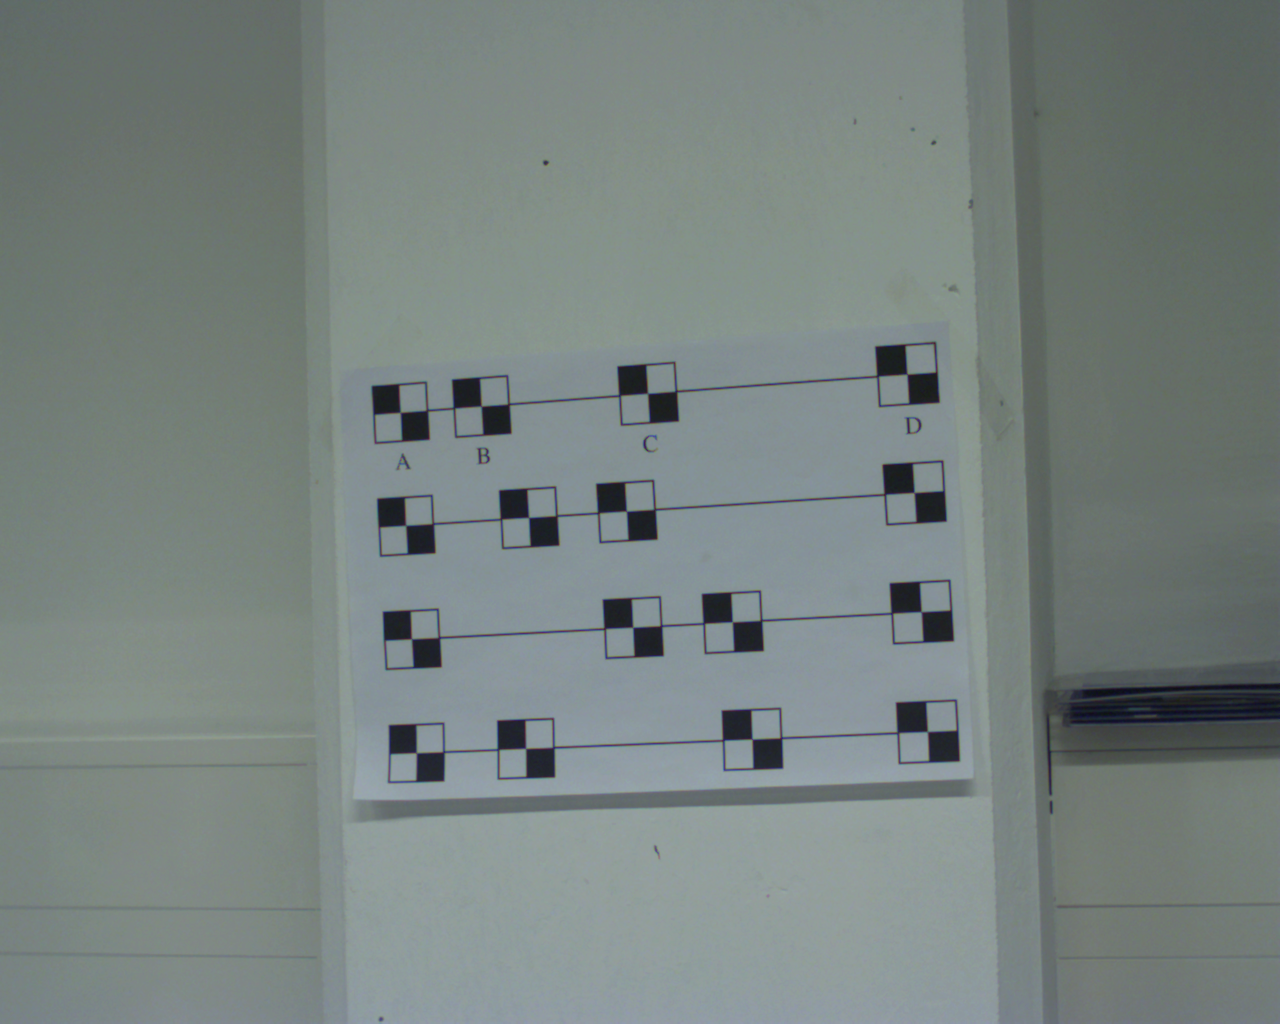
\includegraphics[width=48mm]{./Bildg_Messtechnik_Lab/CrossRatio/images/image_b4.png}\\
(g) $12.5mm$ & (h) $12.5mm$ & (i) $12.5mm$\\[6pt]
 \multicolumn{3}{c}{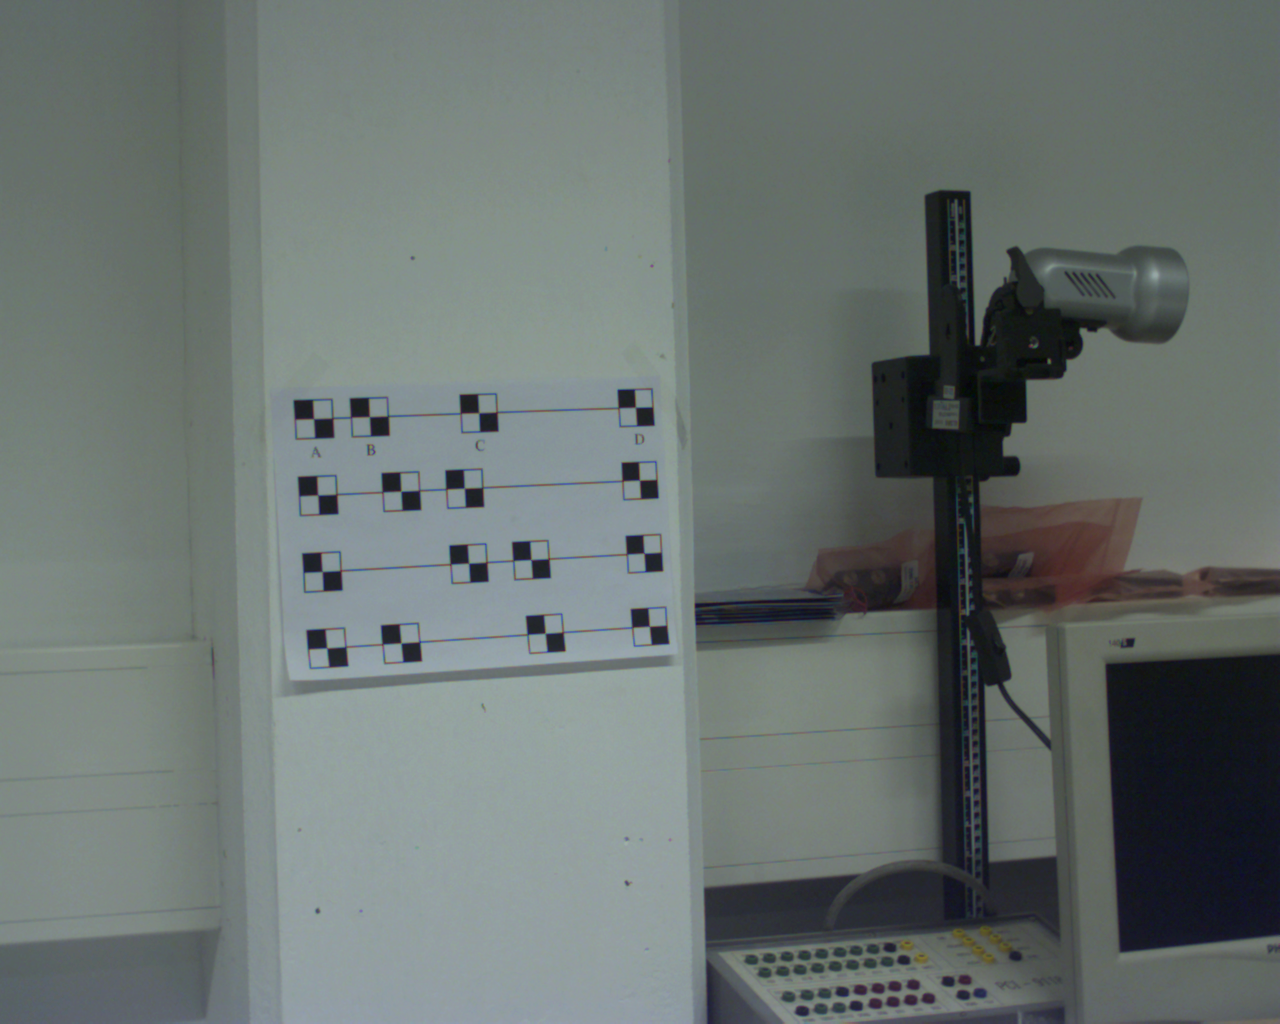
\includegraphics[width=48mm]{./Bildg_Messtechnik_Lab/CrossRatio/images/image_b5.png}} \\[6pt]
 \multicolumn{3}{c}{(j) $\rightarrow\infty$}
\end{tabular}
\caption{All 10 taken images of the scene}
\label{fig:cornermark_images}
\end{figure}

%%%
%%% end main document
%%%
%%%%%%%%%%%%%%%%%%%%%%%%%%%%%%%%%%%%%%%%%%%%%%%%%%%%%%%%%%%%%%%%%%%%%%%%%%%%%%%%

% \appendix  %% include it, if something (bibliography, index, ...) follows below

%%%%%%%%%%%%%%%%%%%%%%%%%%%%%%%%%%%%%%%%%%%%%%%%%%%%%%%%%%%%%%%%%%%%%%%%%%%%%%%%
%%%
%%% bibliography
%%%
%%% available styles: abbrv, acm, alpha, apalike, ieeetr, plain, siam, unsrt
%%%
% \bibliographystyle{plain}

%%% name of the bibliography file without .bib
%%% e.g.: literatur.bib -> \bibliography{literatur}
% \bibliography{FIXXME}

\end{document}
%%% }}}
%%% END OF FILE
%%%%%%%%%%%%%%%%%%%%%%%%%%%%%%%%%%%%%%%%%%%%%%%%%%%%%%%%%%%%%%%%%%%%%%%%%%%%%%%%
%%% Notice!
%%% This file uses the outline-mode of emacs and the foldmethod of Vim.
%%% Press 'zi' to unfold the file in Vim.
%%% See ':help folding' for more information.
%%%%%%%%%%%%%%%%%%%%%%%%%%%%%%%%%%%%%%%%%%%%%%%%%%%%%%%%%%%%%%%%%%%%%%%%%%%%%%%%
%% Local Variables:
%% mode: outline-minor
%% OPToutline-regexp: "%% .*"
%% OPTeval: (hide-body)
%% emerge-set-combine-versions-template: "%a\n%b\n"
%% End:
%% vim:foldmethod=marker
